\documentclass[preprint,10pt]{sigplanconf}
%\documentclass{sigplanconf}

\usepackage{amssymb}
\usepackage{amsthm}
\usepackage{breakurl}             % Not needed if you use pdflatex only.
\usepackage{color}
\usepackage{epsfig}
\usepackage{esvect}
\usepackage{listings}
\usepackage{mathpartir}
\usepackage{MnSymbol}
\usepackage{multirow}
\usepackage{rotating}

\lstdefinestyle{C++}{language=C++,%
showstringspaces=false,
  columns=fullflexible,
  escapechar=@,
  basicstyle=\sffamily,
%  commentstyle=\rmfamily\itshape,
  moredelim=**[is][\color{white}]{~}{~},
  morekeywords={concept,requires,noexcept},
  literate={[<]}{{\textless}}1      {[>]}{{\textgreater}}1 %
           {<}{{$\langle$}}1        {>}{{$\rangle$}}1 %
           {<=}{{$\leq$}}1          {>=}{{$\geq$}}1          
           {==}{{$==$}}2            {!=}{{$\neq$}}1 %
           {=>}{{$\Rightarrow\;$}}1 {->}{{$\rightarrow{}$}}1 %
           {<:}{{$\subtype{}\ $}}1  {<-}{{$\leftarrow$}}1 %
           {s1;}{{$s_1$;}}3 {s2;}{{$s_2$;}}3 {s3;}{{$s_3$;}}3 {s4;}{{$s_4$;}}3 {s5;}{{$s_5$;}}3 {s6;}{{$s_6$;}}3 {s7;}{{$s_7$;}}3 {sn;}{{$s_n$;}}3 {si;}{{$s_i$;}}3%
           {P1}{{$P_1$}}2 {P2}{{$P_2$}}2 {P3}{{$P_3$}}2 {P4}{{$P_4$}}2 {P5}{{$P_5$}}2 {P6}{{$P_6$}}2 {P7}{{$P_7$}}2 {Pn}{{$P_n$}}2 {Pi}{{$P_i$}}2%
           {D1}{{$D_1$}}2 {D2}{{$D_2$}}2 {D3}{{$D_3$}}2 {D4}{{$D_4$}}2 {D5}{{$D_5$}}2 {D6}{{$D_6$}}2 {D7}{{$D_7$}}2 {Dn}{{$D_n$}}2 {Di}{{$D_i$}}2%
           {T1}{{$T_1$}}2 {T2}{{$T_2$}}2 {T3}{{$T_3$}}2 {T4}{{$T_4$}}2 {T5}{{$T_5$}}2 {T6}{{$T_6$}}2 {T7}{{$T_7$}}2 {Tn}{{$T_n$}}2 {Ti}{{$T_i$}}2 {Tm}{{$T_m$}}2%
           {e1}{{$e_1$}}2 {e2}{{$e_2$}}2 {e3}{{$e_3$}}2 {e4}{{$e_4$}}2%
           {E1}{{$E_1$}}2 {E2}{{$E_2$}}2 {E3}{{$E_3$}}2 {E4}{{$E_4$}}2%
           {m_e1}{{$m\_e_1$}}4 {m_e2}{{$m\_e_2$}}4 {m_e3}{{$m\_e_3$}}4 {m_e4}{{$m\_e_4$}}4%
           {Divide}{{Divide}}6 %
           {Times}{{Times}}5 %
           {Match}{{\emph{Match}}}5 %
           {Case}{{\emph{Case}}}4 %
           {Qua}{{\emph{Qua}}}3 %
           {When}{{\emph{When}}}4 %
           {Otherwise}{{\emph{Otherwise}}}9 %
           {EndMatch}{{\emph{EndMatch}}}8 %
           {CM}{{\emph{CM}}}2 {KS}{{\emph{KS}}}2 {KV}{{\emph{KV}}}2 %
           {EuclideanDomain}{\concept{EuclideanDomain}}{15}  %
           {LazyExpression}{\concept{LazyExpression}}{14}    %
           {Polymorphic}{\concept{Polymorphic}}{11}          %
           {Convertible}{\concept{Convertible}}{11}          %
           {Integral}{\concept{Integral}}8                   %
           {SameType}{\concept{SameType}}8                   %
           {Pattern}{\concept{Pattern}}7                     %
           {Regular}{\concept{Regular}}7                     %
           {Object}{\concept{Object}}6                       %
           {Field}{\concept{Field}}5                         %
}
\lstset{style=C++}

\lstdefinestyle{Caml}{language=Caml,%
  morekeywords={when}
}

\lstdefinestyle{Haskell}{language=Haskell,%
  morekeywords={out,view,real}
}

\DeclareMathOperator*{\argmin}{arg\,min}
\DeclareRobustCommand{\Cpp}{C\texttt{++}}
\DeclareRobustCommand{\code}[1]{{\lstinline[breaklines=false,escapechar=@]{#1}}}
\DeclareRobustCommand{\codebr}[1]{{\lstinline[breaklines=true]{#1}}}
\DeclareRobustCommand{\codehaskell}[1]{{\lstinline[breaklines=false,language=Haskell]{#1}}}
\DeclareRobustCommand{\codeocaml}[1]{{\lstinline[breaklines=false,language=Caml]{#1}}}
\DeclareRobustCommand{\concept}[1]{{\small\textsc{#1}}}
\newcommand{\exclude}[1]{}
\newcommand{\halfline}{\vspace{-1.5ex}}

\newtheorem{lemma}{Lemma}
\newtheorem{theorem}{Theorem}
\newtheorem{corollary}{Corollary}

%% grammar commands
\newcommand{\Rule}[1]{{\rmfamily\itshape{#1}}}
\newcommand{\Alt}{\ensuremath{|}}
\newcommand{\is}{$::=$}
\newcommand{\subtype}{\ensuremath{<:}}
\newcommand{\lazyevals}{\Downarrow}
\newcommand{\evals}{\Rightarrow}
\newcommand{\evalspp}{\Rightarrow^+}
\newcommand{\DynCast}[2]{\ensuremath{dc\langle{#1}\rangle({#2})}}
\newcommand{\nullptr}{\ensuremath{\bot}}

\newcommand{\f}[1]{{ {{#1\%}}}}
\newcommand{\s}[1]{{ {\bf \underline{#1\%}}}}
\newcommand{\n}[1]{{ {\bf ~ ~ ~ ~ }}}
\newcommand{\Opn}{{\scriptsize {\bf Open}}}
\newcommand{\Cls}{{\scriptsize {\bf Tag}}}
\newcommand{\Unn}{{\scriptsize {\bf Union}}}

%\newcommand{\gwNGPp}{\n{}}
%\newcommand{\gwNGKp}{\n{}}
 \newcommand{\gwNGUp}{\n{}}
%\newcommand{\gwNSPp}{\n{}}
%\newcommand{\gwNSKp}{\n{}}
 \newcommand{\gwNSUp}{\n{}}
%\newcommand{\vwNGPp}{\n{}}
%\newcommand{\vwNGKp}{\n{}}
 \newcommand{\vwNGUp}{\n{}}
%\newcommand{\vwNSPp}{\n{}}
%\newcommand{\vwNSKp}{\n{}}
 \newcommand{\vwNSUp}{\n{}}
%\newcommand{\vxNGPp}{\n{}}
%\newcommand{\vxNGKp}{\n{}}
 \newcommand{\vxNGUp}{\n{}}
%\newcommand{\vxNSPp}{\n{}}
%\newcommand{\vxNSKp}{\n{}}
 \newcommand{\vxNSUp}{\n{}}

%\newcommand{\gwNGPq}{\n{}}
%\newcommand{\gwNGKq}{\n{}}
 \newcommand{\gwNGUq}{\n{}}
%\newcommand{\gwNSPq}{\n{}}
%\newcommand{\gwNSKq}{\n{}}
 \newcommand{\gwNSUq}{\n{}}
%\newcommand{\vwNGPq}{\n{}}
%\newcommand{\vwNGKq}{\n{}}
 \newcommand{\vwNGUq}{\n{}}
%\newcommand{\vwNSPq}{\n{}}
%\newcommand{\vwNSKq}{\n{}}
 \newcommand{\vwNSUq}{\n{}}
%\newcommand{\vxNGPq}{\n{}}
%\newcommand{\vxNGKq}{\n{}}
 \newcommand{\vxNGUq}{\n{}}
%\newcommand{\vxNSPq}{\n{}}
%\newcommand{\vxNSKq}{\n{}}
 \newcommand{\vxNSUq}{\n{}}

%\newcommand{\gwNGPn}{\n{}}
%\newcommand{\gwNGKn}{\n{}}
 \newcommand{\gwNGUn}{\n{}}
%\newcommand{\gwNSPn}{\n{}}
%\newcommand{\gwNSKn}{\n{}}
 \newcommand{\gwNSUn}{\n{}}
%\newcommand{\vwNGPn}{\n{}}
%\newcommand{\vwNGKn}{\n{}}
 \newcommand{\vwNGUn}{\n{}}
%\newcommand{\vwNSPn}{\n{}}
%\newcommand{\vwNSKn}{\n{}}
 \newcommand{\vwNSUn}{\n{}}
%\newcommand{\vxNGPn}{\n{}}
%\newcommand{\vxNGKn}{\n{}}
 \newcommand{\vxNGUn}{\n{}}
%\newcommand{\vxNSPn}{\n{}}
%\newcommand{\vxNSKn}{\n{}}
 \newcommand{\vxNSUn}{\n{}}


%\newcommand{\gwYGPp}{\n{}}
% \newcommand{\gwYGKp}{\n{}}
 \newcommand{\gwYGUp}{\n{}}
%\newcommand{\gwYSPp}{\n{}}
% \newcommand{\gwYSKp}{\n{}}
 \newcommand{\gwYSUp}{\n{}}
%\newcommand{\vwYGPp}{\n{}}
% \newcommand{\vwYGKp}{\n{}}
 \newcommand{\vwYGUp}{\n{}}
%\newcommand{\vwYSPp}{\n{}}
% \newcommand{\vwYSKp}{\n{}}
 \newcommand{\vwYSUp}{\n{}}
%\newcommand{\vxYGPp}{\n{}}
% \newcommand{\vxYGKp}{\n{}}
 \newcommand{\vxYGUp}{\n{}}
%\newcommand{\vxYSPp}{\n{}}
% \newcommand{\vxYSKp}{\n{}}
 \newcommand{\vxYSUp}{\n{}}

%\newcommand{\gwYGPq}{\n{}}
% \newcommand{\gwYGKq}{\n{}}
 \newcommand{\gwYGUq}{\n{}}
%\newcommand{\gwYSPq}{\n{}}
% \newcommand{\gwYSKq}{\n{}}
 \newcommand{\gwYSUq}{\n{}}
%\newcommand{\vwYGPq}{\n{}}
% \newcommand{\vwYGKq}{\n{}}
 \newcommand{\vwYGUq}{\n{}}
%\newcommand{\vwYSPq}{\n{}}
% \newcommand{\vwYSKq}{\n{}}
 \newcommand{\vwYSUq}{\n{}}
%\newcommand{\vxYGPq}{\n{}}
% \newcommand{\vxYGKq}{\n{}}
 \newcommand{\vxYGUq}{\n{}}
%\newcommand{\vxYSPq}{\n{}}
% \newcommand{\vxYSKq}{\n{}}
 \newcommand{\vxYSUq}{\n{}}

%\newcommand{\gwYGPn}{\n{}}
% \newcommand{\gwYGKn}{\n{}}
 \newcommand{\gwYGUn}{\n{}}
%\newcommand{\gwYSPn}{\n{}}
% \newcommand{\gwYSKn}{\n{}}
 \newcommand{\gwYSUn}{\n{}}
%\newcommand{\vwYGPn}{\n{}}
% \newcommand{\vwYGKn}{\n{}}
 \newcommand{\vwYGUn}{\n{}}
%\newcommand{\vwYSPn}{\n{}}
% \newcommand{\vwYSKn}{\n{}}
 \newcommand{\vwYSUn}{\n{}}
%\newcommand{\vxYGPn}{\n{}}
% \newcommand{\vxYGKn}{\n{}}
 \newcommand{\vxYGUn}{\n{}}
%\newcommand{\vxYSPn}{\n{}}
% \newcommand{\vxYSKn}{\n{}}
 \newcommand{\vxYSUn}{\n{}}

 \newcommand{\GwNGPp}{\n{}}
 \newcommand{\GwNGKp}{\n{}}
 \newcommand{\GwNGUp}{\n{}}
 \newcommand{\GwNSPp}{\n{}}
 \newcommand{\GwNSKp}{\n{}}
 \newcommand{\GwNSUp}{\n{}}
%\newcommand{\VwNGPp}{\n{}}
%\newcommand{\VwNGKp}{\n{}}
 \newcommand{\VwNGUp}{\n{}}
%\newcommand{\VwNSPp}{\n{}}
%\newcommand{\VwNSKp}{\n{}}
 \newcommand{\VwNSUp}{\n{}}
%\newcommand{\VxNGPp}{\n{}}
%\newcommand{\VxNGKp}{\n{}}
 \newcommand{\VxNGUp}{\n{}}
%\newcommand{\VxNSPp}{\n{}}
%\newcommand{\VxNSKp}{\n{}}
 \newcommand{\VxNSUp}{\n{}}

 \newcommand{\GwNGPq}{\n{}}
 \newcommand{\GwNGKq}{\n{}}
 \newcommand{\GwNGUq}{\n{}}
 \newcommand{\GwNSPq}{\n{}}
 \newcommand{\GwNSKq}{\n{}}
 \newcommand{\GwNSUq}{\n{}}
%\newcommand{\VwNGPq}{\n{}}
%\newcommand{\VwNGKq}{\n{}}
 \newcommand{\VwNGUq}{\n{}}
%\newcommand{\VwNSPq}{\n{}}
%\newcommand{\VwNSKq}{\n{}}
 \newcommand{\VwNSUq}{\n{}}
%\newcommand{\VxNGPq}{\n{}}
%\newcommand{\VxNGKq}{\n{}}
 \newcommand{\VxNGUq}{\n{}}
%\newcommand{\VxNSPq}{\n{}}
%\newcommand{\VxNSKq}{\n{}}
 \newcommand{\VxNSUq}{\n{}}

 \newcommand{\GwNGPn}{\n{}}
 \newcommand{\GwNGKn}{\n{}}
 \newcommand{\GwNGUn}{\n{}}
 \newcommand{\GwNSPn}{\n{}}
 \newcommand{\GwNSKn}{\n{}}
 \newcommand{\GwNSUn}{\n{}}
%\newcommand{\VwNGPn}{\n{}}
%\newcommand{\VwNGKn}{\n{}}
 \newcommand{\VwNGUn}{\n{}}
%\newcommand{\VwNSPn}{\n{}}
%\newcommand{\VwNSKn}{\n{}}
 \newcommand{\VwNSUn}{\n{}}
%\newcommand{\VxNGPn}{\n{}}
%\newcommand{\VxNGKn}{\n{}}
 \newcommand{\VxNGUn}{\n{}}
%\newcommand{\VxNSPn}{\n{}}
%\newcommand{\VxNSKn}{\n{}}
 \newcommand{\VxNSUn}{\n{}}


 \newcommand{\GwYGPp}{\n{}}
 \newcommand{\GwYGKp}{\n{}}
 \newcommand{\GwYGUp}{\n{}}
 \newcommand{\GwYSPp}{\n{}}
 \newcommand{\GwYSKp}{\n{}}
 \newcommand{\GwYSUp}{\n{}}
%\newcommand{\VwYGPp}{\n{}}
% \newcommand{\VwYGKp}{\n{}}
 \newcommand{\VwYGUp}{\n{}}
%\newcommand{\VwYSPp}{\n{}}
% \newcommand{\VwYSKp}{\n{}}
 \newcommand{\VwYSUp}{\n{}}
%\newcommand{\VxYGPp}{\n{}}
% \newcommand{\VxYGKp}{\n{}}
 \newcommand{\VxYGUp}{\n{}}
%\newcommand{\VxYSPp}{\n{}}
% \newcommand{\VxYSKp}{\n{}}
 \newcommand{\VxYSUp}{\n{}}

 \newcommand{\GwYGPq}{\n{}}
 \newcommand{\GwYGKq}{\n{}}
 \newcommand{\GwYGUq}{\n{}}
 \newcommand{\GwYSPq}{\n{}}
 \newcommand{\GwYSKq}{\n{}}
 \newcommand{\GwYSUq}{\n{}}
%\newcommand{\VwYGPq}{\n{}}
% \newcommand{\VwYGKq}{\n{}}
 \newcommand{\VwYGUq}{\n{}}
%\newcommand{\VwYSPq}{\n{}}
% \newcommand{\VwYSKq}{\n{}}
 \newcommand{\VwYSUq}{\n{}}
%\newcommand{\VxYGPq}{\n{}}
% \newcommand{\VxYGKq}{\n{}}
 \newcommand{\VxYGUq}{\n{}}
%\newcommand{\VxYSPq}{\n{}}
% \newcommand{\VxYSKq}{\n{}}
 \newcommand{\VxYSUq}{\n{}}

 \newcommand{\GwYGPn}{\n{}}
 \newcommand{\GwYGKn}{\n{}}
 \newcommand{\GwYGUn}{\n{}}
 \newcommand{\GwYSPn}{\n{}}
 \newcommand{\GwYSKn}{\n{}}
 \newcommand{\GwYSUn}{\n{}}
%\newcommand{\VwYGPn}{\n{}}
% \newcommand{\VwYGKn}{\n{}}
 \newcommand{\VwYGUn}{\n{}}
%\newcommand{\VwYSPn}{\n{}}
% \newcommand{\VwYSKn}{\n{}}
 \newcommand{\VwYSUn}{\n{}}
%\newcommand{\VxYGPn}{\n{}}
% \newcommand{\VxYGKn}{\n{}}
 \newcommand{\VxYGUn}{\n{}}
%\newcommand{\VxYSPn}{\n{}}
% \newcommand{\VxYSKn}{\n{}}
 \newcommand{\VxYSUn}{\n{}}

% This file defines variables with performance numbers for the table in Evaluation section
% Data from 2011-08-30 
\newcommand{\vwYGKp}{\s{3}}
\newcommand{\vwYGKn}{\s{8}}
\newcommand{\vwYGKq}{\s{11}}
\newcommand{\vwYGPp}{\f{10}}
\newcommand{\vwYGPn}{\f{14}}
\newcommand{\vwYGPq}{\s{0}}
\newcommand{\vwYSKp}{\s{7}}
\newcommand{\vwYSKn}{\s{7}}
\newcommand{\vwYSKq}{\s{10}}
\newcommand{\vwYSPp}{\f{10}}
\newcommand{\vwYSPn}{\f{14}}
\newcommand{\vwYSPq}{\s{0}}
\newcommand{\vwNGKp}{\f{35}}
\newcommand{\vwNGKn}{\s{6}}
\newcommand{\vwNGKq}{\s{5}}
\newcommand{\vwNGPp}{\f{1}}
\newcommand{\vwNGPn}{\s{1}}
\newcommand{\vwNGPq}{\s{10}}
\newcommand{\vwNSKp}{\f{133}}
\newcommand{\vwNSKn}{\f{25}}
\newcommand{\vwNSKq}{\f{59}}
\newcommand{\vwNSPp}{\f{1}}
\newcommand{\vwNSPn}{\s{1}}
\newcommand{\vwNSPq}{\s{8}}

\newcommand{\vxYGKp}{\s{61}}
\newcommand{\vxYGKn}{\s{24}}
\newcommand{\vxYGKq}{\s{25}}
\newcommand{\vxYGPp}{\s{24}}
\newcommand{\vxYGPn}{\s{24}}
\newcommand{\vxYGPq}{\s{36}}
\newcommand{\vxYSKp}{\s{79}}
\newcommand{\vxYSKn}{\s{25}}
\newcommand{\vxYSKq}{\s{35}}
\newcommand{\vxYSPp}{\s{9}}
\newcommand{\vxYSPn}{\s{23}}
\newcommand{\vxYSPq}{\f{133}}
\newcommand{\vxNGKp}{\s{8}}
\newcommand{\vxNGKn}{\s{5}}
\newcommand{\vxNGKq}{\s{0}}
\newcommand{\vxNGPp}{\s{33}}
\newcommand{\vxNGPn}{\s{47}}
\newcommand{\vxNGPq}{\s{43}}
\newcommand{\vxNSKp}{\f{38}}
\newcommand{\vxNSKn}{\f{12}}
\newcommand{\vxNSKq}{\f{3}}
\newcommand{\vxNSPp}{\s{27}}
\newcommand{\vxNSPn}{\s{44}}
\newcommand{\vxNSPq}{\s{45}}

\newcommand{\gwYGKp}{\f{88}}
\newcommand{\gwYGKn}{\f{32}}
\newcommand{\gwYGKq}{\f{250}}
\newcommand{\gwYGPp}{\f{67}}
\newcommand{\gwYGPn}{\f{28}}
\newcommand{\gwYGPq}{\f{87}}
\newcommand{\gwYSKp}{\f{79}}
\newcommand{\gwYSKn}{\f{31}}
\newcommand{\gwYSKq}{\f{259}}
\newcommand{\gwYSPp}{\f{67}}
\newcommand{\gwYSPn}{\f{27}}
\newcommand{\gwYSPq}{\f{90}}
\newcommand{\gwNGKp}{\f{116}}
\newcommand{\gwNGKn}{\f{29}}
\newcommand{\gwNGKq}{\f{43}}
\newcommand{\gwNGPp}{\f{55}}
\newcommand{\gwNGPn}{\s{0}}
\newcommand{\gwNGPq}{\f{1}}
\newcommand{\gwNSKp}{\f{216}}
\newcommand{\gwNSKn}{\f{542}}
\newcommand{\gwNSKq}{\f{520}}
\newcommand{\gwNSPp}{\f{55}}
\newcommand{\gwNSPn}{\f{1}}
\newcommand{\gwNSPq}{\f{3}}

\newcommand{\VwYGKp}{\f{16}}
\newcommand{\VwYGKn}{\f{11}}
\newcommand{\VwYGKq}{\f{168}}
\newcommand{\VwYGPp}{\f{10}}
\newcommand{\VwYGPn}{\f{19}}
\newcommand{\VwYGPq}{\f{153}}
\newcommand{\VwYSKp}{\f{31}}
\newcommand{\VwYSKn}{\f{24}}
\newcommand{\VwYSKq}{\f{185}}
\newcommand{\VwYSPp}{\f{10}}
\newcommand{\VwYSPn}{\f{18}}
\newcommand{\VwYSPq}{\f{153}}
\newcommand{\VwNGKp}{\f{61}}
\newcommand{\VwNGKn}{\f{18}}
\newcommand{\VwNGKq}{\f{13}}
\newcommand{\VwNGPp}{\f{4}}
\newcommand{\VwNGPn}{\s{17}}
\newcommand{\VwNGPq}{\s{9}}
\newcommand{\VwNSKp}{\f{124}}
\newcommand{\VwNSKn}{\f{43}}
\newcommand{\VwNSKq}{\f{34}}
\newcommand{\VwNSPp}{\f{4}}
\newcommand{\VwNSPn}{\s{18}}
\newcommand{\VwNSPq}{\f{3}}
               
\newcommand{\VxYGKp}{\s{5}}
\newcommand{\VxYGKn}{\s{2}}
\newcommand{\VxYGKq}{\f{132}}
\newcommand{\VxYGPp}{\s{5}}
\newcommand{\VxYGPn}{\s{5}}
\newcommand{\VxYGPq}{\f{130}}
\newcommand{\VxYSKp}{\s{9}}
\newcommand{\VxYSKn}{\s{10}}
\newcommand{\VxYSKq}{\f{118}}
\newcommand{\VxYSPp}{\s{6}}
\newcommand{\VxYSPn}{\s{6}}
\newcommand{\VxYSPq}{\f{145}}
\newcommand{\VxNGKp}{\f{20}}
\newcommand{\VxNGKn}{\f{7}}
\newcommand{\VxNGKq}{\f{34}}
\newcommand{\VxNGPp}{\s{14}}
\newcommand{\VxNGPn}{\s{27}}
\newcommand{\VxNGPq}{\f{2}}
\newcommand{\VxNSKp}{\f{47}}
\newcommand{\VxNSKn}{\f{16}}
\newcommand{\VxNSKq}{\f{14}}
\newcommand{\VxNSPp}{\s{0}}
\newcommand{\VxNSPn}{\s{27}}
\newcommand{\VxNSPq}{\f{1}}


\newsavebox{\sembox}
\newlength{\semwidth}
\newlength{\boxwidth}

\newcommand{\Sem}[1]{%
\sbox{\sembox}{\ensuremath{#1}}%
\settowidth{\semwidth}{\usebox{\sembox}}%
\sbox{\sembox}{\ensuremath{\left[\usebox{\sembox}\right]}}%
\settowidth{\boxwidth}{\usebox{\sembox}}%
\addtolength{\boxwidth}{-\semwidth}%
\left[\hspace{-0.3\boxwidth}%
\usebox{\sembox}%
\hspace{-0.3\boxwidth}\right]%
}

\newcommand{\authormodification}[2]{{\color{#1}#2}}
\newcommand{\ys}[1]{\authormodification{blue}{#1}}
\newcommand{\bs}[1]{\authormodification{red}{#1}}
\newcommand{\gdr}[1]{\authormodification{magenta}{#1}}

\begin{document}

%\conferenceinfo{PLDI 2012}{Beijing, China} 
%\copyrightyear{2012} 
%\copyrightdata{[to be supplied]} 

\titlebanner{Draft for OOPSLA 2012} % These are ignored unless
\preprintfooter{Y.Solodkyy, G.Dos Reis, B.Stroustrup: Open and Efficient Type Switch for C++}   % 'preprint' option specified.

\title{Open and Efficient Type Switch for C++}
%\subtitle{your \code{visit}, Jim, is not \code{accept}able anymore}
%\subtitle{\code{accepting} aint no \code{visit}ors}

\authorinfo{Yuriy Solodkyy\and Gabriel Dos Reis\and Bjarne Stroustrup}
           {Texas A\&M University\\ Texas, USA}
           {\{yuriys,gdr,bs\}@cse.tamu.edu}

\maketitle

\begin{abstract}
%Selecting operations based on a type of an object determined at run-time is key 
%to many object-oriented and functional programming techniques. We present 
%techniques that can implement efficient type switching, type testing, pattern 
%matching, predicate dispatch, multi-methods in a compiler or a library. The 
%techniques are general and cope well with C++ multiple inheritance.
%
%Our library-only implementation provides a functional programming style notation 
%to the programmer. It outperforms the visitor design pattern, as commonly used 
%for type-casing scenarios in C++. For many use cases it equals or outperforms 
%equivalent code in languages with built-in type switching constructs, such as 
%OCaml. We find the pattern-based library code easier to read and write and more 
%expressive than hand-coded visitors. The library is non-intrusive and does not have 
%extensibility restrictions. It also avoids control inversion characteristic to 
%visitors.
% 
%The library was motivated by and is used for applications involving large, 
%typed, abstract syntax trees. Being a library only solution allows us to use 
%production quality compilers and tool chains for our experiments and our 
%intended applications.

Selecting operations based on the run-time type of an object is key to many
object-oriented and functional programming techniques. We present a technique
for implementing open and efficient type-switching for hierarchical extensible 
data types. The technique is general and copes well with C++ multiple 
inheritance.
 
To simplify experimentation and gain realistic preformance using production-quality
compilers and tool chains, we implement our type swich constructs as an ISO C++11 library.
Our library-only implementation provides concise notation and
outperforms the visitor design pattern, commonly used for type-casing
scenarios in object-oriented programs. For many uses, it equals or outperforms
equivalent code in languages with built-in type-switching constructs, such as
OCaml and Haskell. The type-switching code is easier to use and is more expressive 
than hand-coded visitors. The library is non-intrusive and circumvents most of
extensibility restrictions typical of visitor design pattern. 
It was motivated by applications involving large, typed, abstract
syntax trees. 

%We present techniques that can be used in a compiler or library setting to 
%efficiently implement type switching, type testing, pattern matching, predicate 
%dispatch, multi-methods and other facilities that depend on the run-time type 
%of an argument. The techniques cope well with multiple inheritance in C++, 
%however they are not specific to C++ and can be adapted to implement 
%similar facilities in other languages.
%
%Our library-only implementation of a type switch based on these techniques equals 
%or outperforms the visitor design pattern, as commonly used for type-casing 
%scenarios in C++. For many use cases, it equals or outperforms equivalent 
%code in languages with built-in type-switching constructs. While remaining a 
%library-only solution, such a facility better addresses the expression problem 
%than the visitor design pattern does: it is non-intrusive and does not have 
%extensibility restrictions. It also avoids the control inversion characteristic to 
%visitors, thereby making the code significantly more concise and easier to comprehend.
%The library was motivated by and is used for applications involving large, 
%typed abstract syntax trees.
\end{abstract}

\category{D}{1}{5}
\category{D}{3}{3}

\terms
Languages, Design

\keywords
Type Switch, Typecase, Visitor Design Pattern, Memoization, C++

\section{Introduction} %%%%%%%%%%%%%%%%%%%%%%%%%%%%%%%%%%%%%%%%%%%%%%%%%%%%%%%%%
\label{sec:intro}

%Motivate the problem
%Give a summary of the paper: what you did and how
%Explicitly state your contribution

Algebraic data types as seen in functional languages are closed and their 
variants are disjoint. This allows for easy addition of new functions through 
case analysis as well as their efficient implementation. Data types in 
object-oriented languages are extensible and hierarchical (non-disjoint), which 
significantly complicates the addition of new functions. Existing approaches to 
case analysis on such types are either efficient or open, but not both. Truly 
open approaches, which allow for independent extensibility, modular 
type-checking and dynamic linking, rely on class-membership testing combined 
with a decision tree. Efficient approaches rely on sealing either the class 
hierarchy or the set of functions, which looses extensibility. Consider a simple 
expression language:

\begin{lstlisting}
@$exp$ \is{} $val$ \Alt{} $exp+exp$ \Alt{} $exp-exp$ \Alt{} $exp*exp$ \Alt{} $exp/exp$@
\end{lstlisting}

\noindent 
In an object-oriented language without direct support for algebraic data types, 
the type representing an expression-tree in the language will typically be 
encoded as an abstract base class, listing the (sealed set of) allowed virtual 
functions, with derived classes representing variants:

\begin{lstlisting}[keepspaces,columns=flexible]
struct Expr { virtual @$\sim$@Expr() {} };
struct Value  : Expr { int value; };
struct Plus   : Expr { Expr* e1; Expr* e2; }; // ...
\end{lstlisting}

\noindent
A simple evaluator for this language can be implemented with the aid of a
virtual function \code{eval()} declared in the base class \code{Expr}. 
The approach is \emph{intrusive}, as we will have to modify the base class every 
time we would like to add a function. A less-intrusive solution to the 
extensibility of functions can be achieved with \emph{visitor design 
pattern}~\cite{DesignPatterns1993}. That solution, however, is not open as it 
restricts extensibility of classes.

Our solution overcomes extensibility problems of both functions and 
types by allowing external introspection of objects with a type switch:

\begin{lstlisting}[keepspaces,columns=flexible]
int eval(const Expr* e)
{
  Match(e)
    Case(Value,  n)    return n;
    Case(Plus,   a, b) return eval(a) + eval(b);
    Case(Minus,  a, b) return eval(a) - eval(b);
    Case(Times,  a, b) return eval(a) * eval(b);
    Case(Divide, a, b) return eval(a) / eval(b);
  EndMatch
}
\end{lstlisting}

\noindent
The syntax is provided without any external tool support. Instead we rely on a 
few C++0x features~\cite{C++0x}, template meta-programming, and macros. It runs 
about as fast as the OCaml version (\textsection\ref{sec:ocaml}), and, depending 
on the usage scenario, compiler and underlying hardware, comes close or 
outperforms the handcrafted C++ code based on the \emph{visitor design pattern} 
(\textsection\ref{sec:eval}). The mapping of members to matching positions that 
the user has to provide to make the above example fully functional is 
omitted~\cite[\textsection 3.1]{TR}.

%\subsection{Summary}

We present techniques based on memoization (\textsection\ref{sec:copc}) and 
class precedence list (\textsection\ref{sec:cotc}) that can be used to
implement type switching efficiently based on the run-time type of the
argument:
  \begin{itemize}
  \setlength{\itemsep}{0pt}
  \setlength{\parskip}{0pt}
  \item The techniques come close and often outperform its de facto contender -- 
        visitor design pattern -- without sacrificing extensibility (\textsection\ref{sec:eval}).
  \item They work in the presence of multiple inheritance, both repeated and 
  shared, as well as in generic code (\textsection\ref{sec:vtblmem}).
  \item The solution is open by construction (\textsection\ref{sec:poets}), 
        non-intrusive, and avoids the control inversion typical for visitors.
  \item It applies to polymorphic (\textsection\ref{sec:vtp}-\ref{sec:vtblmem}) and 
        tagged (\textsection\ref{sec:cotc}) class hierarchies through a unified  
        syntax~\cite[\textsection 8]{TR}.
  \item Our memoization device (\textsection\ref{sec:memdev}) generalizes to 
        other languages and can be used to implement type switching 
        (\textsection\ref{sec:vtblmem}), type testing 
        (\textsection\ref{sec:poets},\cite[\textsection 9]{TR}), predicate dispatch 
        (\textsection\ref{sec:memdev}), and multiple dispatch efficiently.
  \item We list conditions under which virtual table pointers, commonly used in 
        C++ implementations, uniquely identify the exact subobject within the 
        most derived type (\textsection\ref{sec:vtp}).
  \item We also build an efficient cache indexing function for virtual table 
        pointers that minimizes the amount of conflicts 
        (\textsection\ref{sec:sovtp},\ref{sec:moc},\cite[\textsection 5.3.2]{TR}).
  \end{itemize}

\noindent
A practical benefit of our solution is that it can be used right away with any 
compiler with a descent support of C++0x without requiring the installation of 
any additional tools or preprocessors. The solution is a proof of concept that 
sets a minimum threshold for the performance, brevity, clarity and usefulness of 
a language solution for open type switching in C++.

Due to page restrictions, we will only deal here with the part of the library 
concerned with efficient type testing, type identification, and type switching. 
These primitive operations are essential in providing support for type patterns 
and constructor patterns, and their efficiency relative to the visitor design 
pattern might become a major argument for their adoption. We refer the reader to 
technical report~\cite{TR} for more details on our pattern-matching 
library.

%Section~\ref{sec:probl} will motivate the problem as well as discuss some 
%existing solutions and their limitations. Section~\ref{sec:copc} will outline 
%the three techniques that comprise our solution, while the 
%section~\ref{sec:eval} will evaluate their performance. Related work is 
%discussed in Section~\ref{sec:rw}, followed by concluding remarks in 
%Section~\ref{sec:cc}.


\section{Overview} %%%%%%%%%%%%%%%%%%%%%%%%%%%%%%%%%%%%%%%%%%%%%%%%%%
\label{sec:over}

A \emph{class hierarchy} is a partially ordered set $(H,\subtype)$ where $H$ is a potentially open set 
of classes and $\subtype$ is a reflexive, transitive and anti-symmetric 
\emph{subtyping relation} on $H$. We use \emph{class} and \emph{type}  
interchangeably.
% as the exact distinction is not important for this discussion. 
When two classes are in a subtyping relation $D \subtype B$, the class $D$
is said to be a (possibly indirect) \emph{derived class} (or subtype) of $B$;
the class $B$ is called a (possibly indirect) \emph{base class}
(or supertype) of $D$.
 %When the transitive reduction 
%$\subtypeD$ of $\subtype$ is a function, $H$ is usually referred to as 
%\emph{hierarchy} to indicate single inheritance.

The %\emph{most-derived type of an object} also known as the 
\emph{dynamic type of an object} is the type used to create it.
The \emph{static type of an expression} is the type of that expression
as given by the static semantics.%, i.e. the typing rules of expressions.
%  By 
% \emph{dynamic type} of an object we call any base class of the most-derived type.

\subsection{Type Switch}

%This section generalizes pattern matching of closed algebraic datatype values
%to case analysis of hierarchical and extensible datatype values.
In general, a \emph{type switch} or \emph{typecase} is a multiway branch statement 
that distinguishes values based on their type. In a multi-paradigm programming 
language like \Cpp{}, which supports parametric, ad-hoc, and 
subtyping polymorphisms, such a broad definition subsumes numerous different
typecase constructs studied in the literature~\cite{Intensional95,Glew99,OpenShutTypecase05}. 
In this work, we only look at typecasing scenarios based on the class inheritance 
of \Cpp{}, similar to those studied by Glew~\cite{Glew99}. 
% It is possible to generalize type switch
% (the notion, not our implementation) to static polymorphism of \Cpp{} (ad-hoc and 
% parametric polymorphism enabled by overloading and templates) along the line of 
% work introduced by Harper and Morrisett~\cite{Intensional95} and studied in the
% context of closed and extensible solutions by Vytiniotis et 
% al~\cite{OpenShutTypecase05}, but we do not address such a generalization here.
We use the term \emph{type switch} instead of a broader \emph{typecase} to 
stress the run-time nature of the type analysis similar to how regular 
\code{switch}-statement of \Cpp{} performs case analysis of values at run time.

The term \emph{object descriptor} means either a pointer or a reference to 
an object.
Given an object descriptor, called \emph{subject}, of static type \code{S} 
referred to as the \emph{subject type}, and a list of 
\emph{target types} \code{Ti} associated with the branches, a type switch 
statement needs to identify a suitable clause $m$ based on 
the dynamic type \code{D <: S} of the subject as well as a suitable 
conversion that coerces the subject to the target type \code{Tm}.  
Due to multiple inheritance, types \code{Ti} may not all directly
derive from the static type \code{S}. However,
%because of the strong static type safety requirement, 
the type of the applicable clause \code{Tm} will necessarily have to be a 
supertype of the subject's dynamic type \code{D <: Tm}. 
A hypothetical type switch 
statement, not currently supported by \Cpp{}, may look as following:
%
\begin{lstlisting}[keepspaces]
switch (subject) { case T1: s1; ... case Tn: sn; }
\end{lstlisting}
%
\noindent
There is no need for an explicit \emph{default clause} in our setting because 
it is semantically equivalent to a case clause guarded by the 
subject type: \code{case S: s}. The only semantic difference such a choice 
makes is in the treatment of null pointers.
One may naively think that null pointers should be handled by
the default clause.  However, not distinguishing between 
invalid object and valid object of a known static but unknown dynamic type may 
lead to nasty run-time errors.

%\noindent
Similar control structures exist in many programming languages, e.g. 
\emph{match} in Scala~\cite{Scala2nd}, \emph{case} in Haskell~\cite{Haskell98Book} and 
ML~\cite{ML90}, \emph{typecase} in Modula-3~\cite{Modula3TS} and CLOS (as a 
macro), \emph{tagcase} in CLU~\cite{CLURefMan}, \emph{union case} in Algol 68, 
and date back to at least Simula's \emph{Inspect} statement~\cite{Simula67}. 
The statement can, in general, be given numerous plausible semantics:
%
\begin{itemize}
\setlength{\itemsep}{0pt}
\setlength{\parskip}{0pt}
\item \emph{First-fit} semantics will evaluate the first statement $s_i$ such 
      that $T_i$ is a base class of $D$.
\item \emph{Best-fit} semantics will evaluate the statement corresponding to the 
      most-specialized base class $T_i$ of $D$ if it is unique (subject to 
      ambiguity).
\item \emph{Exact-fit} semantics will evaluate statement $s_i$ if $T_i=D$.
\item \emph{All-fit} semantics will evaluate all statements $s_i$ whose guard 
      type $T_i$ is a supertype of $D$ (order of execution has to be defined).
\item \emph{Any-fit} semantics might choose non-deterministically one of the 
      statements enabled by the all-fit semantics.
\end{itemize}
%
The list is not exhaustive and depending on a language, any of them
is a plausible choice. Functional languages, for example, often prefer 
first-fit semantics because it is similar to case analysis in mathematics. 
Object-oriented languages are typically inclined to best-fit semantics due 
to its similarity to overload resolution and run-time dispatch; however, some 
do opt for first-fit semantics to mimic the functional style: e.g. Scala~\cite{Scala2nd}. 
Exact-fit semantics can often be seen in languages supporting discriminated 
union types (sum types): e.g. \emph{variant records} in Pascal, Ada and Modula-2, 
\emph{oneof} and \emph{variant objects} in CLU, \emph{unions} in C and \Cpp{}, etc. 
All-fit and any-fit semantics might be seen in languages based on predicate 
dispatching~\cite{ErnstKC98} or guarded commands~\cite{EWD:EWD472}, where a 
predicate can be seen as a characteristic function of a type, while logical 
implication -- as subtyping.

\subsection{The Expression Problem}

Type switching is related to a more general problem manifesting the differences 
in functional and object-oriented programming styles.
Conventional algebraic datatypes, as found in most functional languages, allow 
for easy addition of new functions on existing data types. However, they fall short 
in extending data types themselves (e.g. with new constructors), which requires 
modifying the source code. Object-oriented languages make 
data type extension trivial through inheritance, but the addition of new 
functions operating on these classes typically requires changes to the class 
definition. This dilemma is known as the \emph{expression problem}~\cite{Cook90,exprproblem}.

\noindent
Classes differ from algebraic data types in two important ways. Firstly, they
are \emph{extensible}, for new variants can be added later by inheriting from
the base class. Secondly, they are \emph{hierarchical} and thus typically 
\emph{non-disjoint} since variants can be inherited from other variants and form 
a subtyping relation between themselves~\cite{Glew99}. In contrast, variants in 
conventional algebraic data types are \emph{disjoint} and \emph{closed}.
Some functional languages e.g. ML2000~\cite{ML2000} and its predecessor, Moby, 
were experimenting with \emph{hierarchical extensible sum types}, which are 
closer to object-oriented classes then algebraic data types are, but, 
interestingly, they provided no %neither traditional nor efficient 
facilities for performing case analysis on them.

Zenger and Odersky refined the expression problem in the context of 
independently extensible solutions~\cite{fool12} as a challenge to find an 
implementation technique that satisfies the following requirements:
%
\begin{itemize}
\setlength{\itemsep}{0pt}
\setlength{\parskip}{0pt}
\item \emph{Extensibility in both dimensions}: It should be possible to add new 
      data variants, while adapting the existing operations accordingly. It 
      should also be possible to introduce new functions. 
\item \emph{Strong static type safety}: It should be impossible to apply a 
      function to a data variant, which it cannot handle. 
\item \emph{No modification or duplication}: Existing code should neither be 
      modified nor duplicated.
\item \emph{Separate compilation}: Neither datatype extensions nor addition of 
      new functions should require re-typechecking the original datatype or 
      existing functions. No safety checks should be deferred until link or 
      runtime.
\item \emph{Independent extensibility}: It should be possible to combine 
      independently developed extensions so that they can be used jointly.
\end{itemize}
%
While these requirements were formulated for extensible data types with 
disjoint variants, object-oriented languages primarily deal with 
hierarchical data types. We thus found it important to state explicitly an 
additional requirement based on the Liskov substitution principle~\cite{Lis87}:
%
\begin{itemize}
\setlength{\itemsep}{0pt}
\setlength{\parskip}{0pt}
\item \emph{Substitutability}: Operations expressed on more general data variants
      should be applicable to ones that are more specific.
      %(the latter being in a subtyping relation with the former).
\end{itemize}

%Depending on the semantics of the language's subtyping relation, 
%substitutability requirement may turn pattern matching into an expensive 
%operation. OCaml, for example, that uses structural subtyping on its object 
%types, does not offer pattern 

\noindent
We will refer to a solution that satisfies all of the above requirements as \emph{open}. 
Numerous solutions have been proposed to dealing with the expression problem in both 
functional~\cite{garrigue-98,LohHinze2006} and object-oriented 
camps~\cite{Palsberg98,Krishnamurthi98,Zenger:2001,runabout}, but very few have 
made their way into one of the mainstream languages. We refer the reader to Zenger 
and Odersky's original manuscript for a discussion of the approaches~\cite{fool12}.
Most of the discussed object-oriented solutions focused on the visitor design pattern and its extensions, 
which even today seem to be the most commonly used approach to dealing with the 
expression problem in object-oriented languages.

A lot has been written about the visitor design pattern~\cite{DesignPatterns1993,Palsberg98,Zenger:2001,Oliveira08}. 
Its advantages include \emph{extensibility of functions}, \emph{speed}, and 
\emph{being a library solution}. Nevertheless, the solution is \emph{intrusive}, 
\emph{specific to hierarchy}, and requires a lot of \emph{boilerplate code} to 
be written. It also introduces \emph{control inversion}, but, most importantly, 
-- \emph{hinders extensibility} of classes.

%In this work we are not trying to solve the expression problem in its full 
%generality. Instead, we concentrate on deficiencies of the visitor design 
%pattern independently of its relation to the expression problem and advocate for 
%a solution that suits object-oriented paradigm better than visitors do.

\subsection{An Open Type Switch}

Type switch alone does not solve the expression problem in the context
of an object-oriented language, for the existing code may have to be 
modified to consider new variants. Relying on a default clause is not 
an acceptable solution in this situation, because often the 
only reasonable default behavior is to raise an exception. 
Zenger and Odersky observed that defaults transform type errors that should
manifest statically into runtime exceptions~\cite{fool12}.
In our experience, newly added variants were more often extending an existing 
variant than creating an entirely disjoint one. In a compiler, for 
example, a new kind of type expression will typically extend a 
\code{TypeExpression} variant, while a new form of annotation will extend an 
\code{Annotation} variant, thus not extending the root \code{ASTNode} directly. 
Due to the substitutability requirement, this new variant will be treated as a 
variant it extends in all the existing code. The functions that will be affected 
by its addition and thus have to be modified will be limited to functions 
directly analyzing the variant it extends and not providing a default behavior.

To account for this subtlety of extensible hierarchical data types, we use a 
term \emph{open type switch} to refer to a type switch that satisfies all the 
requirements of an \emph{open solution to the expression problem} stated above 
except for the \emph{no modification or duplication} requirement. We loosen it 
to allow modification of functions for which the newly added variant becomes a 
disjoint (orthogonal) case not handled by a default clause. We believe that the 
loosened requirement allows us to express pragmatically interesting restrictions 
that developers are willing to live with. Furthermore, 
open type switch overcomes 
all the major shortcomings of the visitor design pattern:
%
\begin{itemize}
\setlength{\itemsep}{0pt}
\setlength{\parskip}{0pt}
\item Case analysis with an open type switch is non-intrusive as it 
      inspects the hierarchy externally and can be applied retroactively. 
\item New variants can be accounted for in the newly written code and will be 
      seen as a base class or default in the existing code.
\item The affected functions are limited to those for which the newly added 
      variant is a disjoint case.
\item The code avoids the control inversion and the need for boilerplate code 
      that visitors introduce, and is thus a more direct expression of the 
      intent.
\end{itemize}

\subsection{\Cpp{} Specifics: Subobjects}
\label{sec:specifics}

\Cpp{} supports two kinds of multiple inheritance: 
\emph{non-virtual} inheritance and \emph{virtual} inheritance~\cite{CPPARM90}. 
The difference between the two only arises in situations where a 
class indirectly inherits from the same base class via more than one path
in its class hierarchy.  Rigorous accounts of \Cpp{} multiple inheritance
semantics use the notion of \emph{subobject}~\cite{RF95}.

\begin{figure}[htbp]
  \centering
    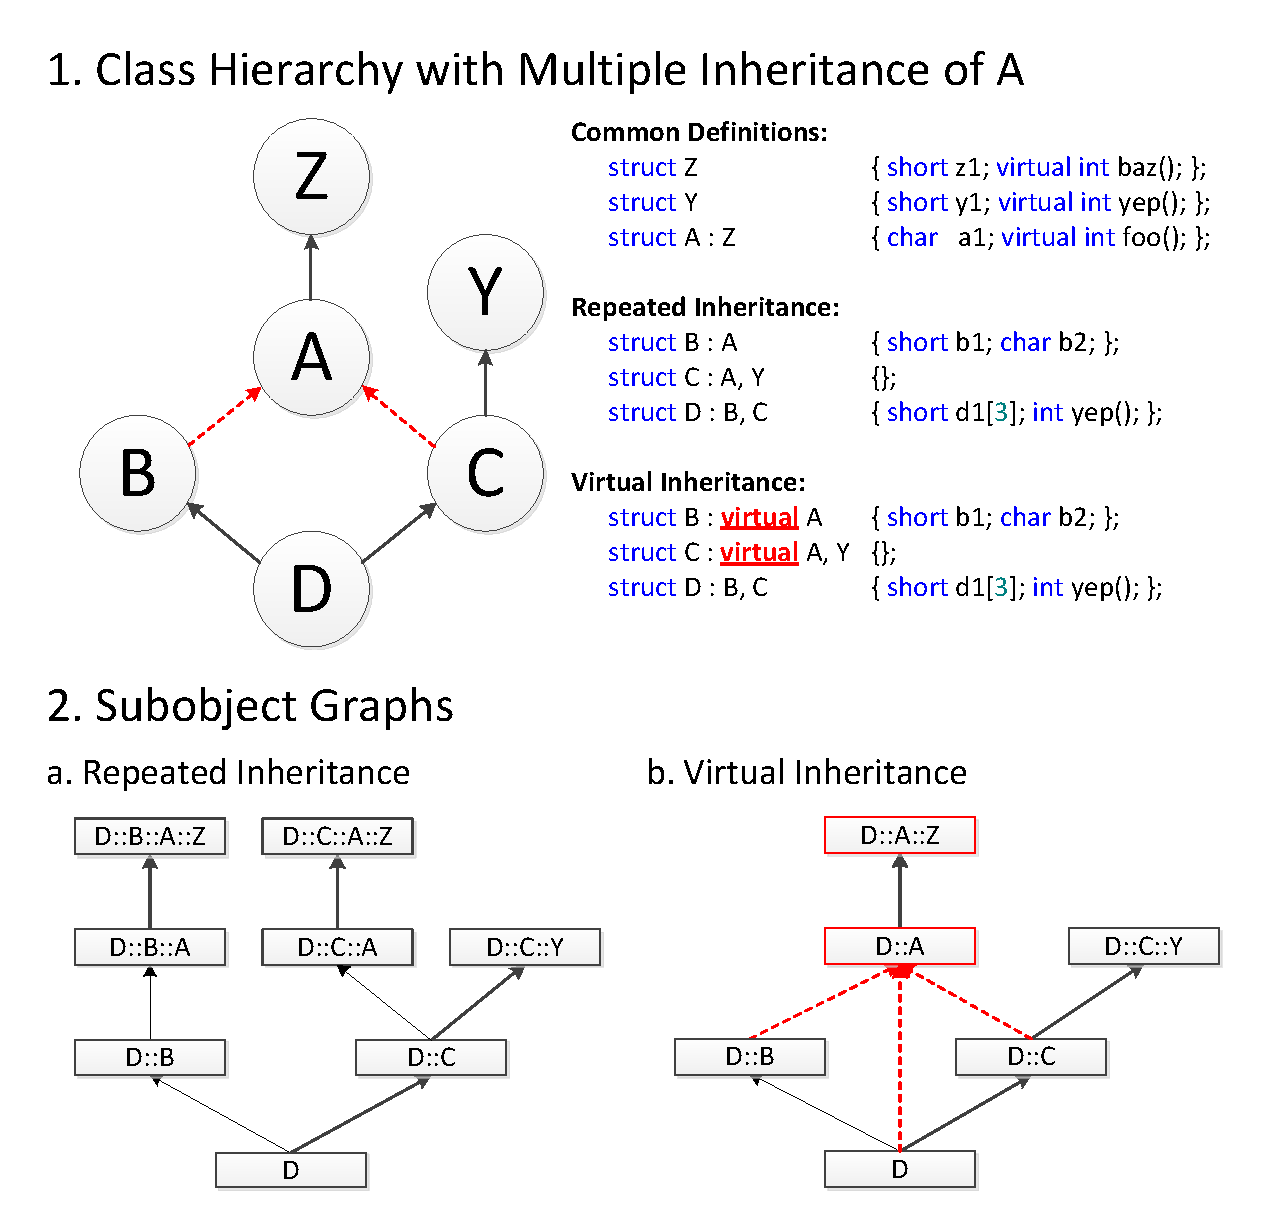
\includegraphics[width=0.47\textwidth]{Inheritance.pdf}
  \caption{Multiple Inheritance in \Cpp{}}
  \label{fig:inheritance}
\end{figure}

\noindent
Consider the simple class hierarchy in Figure~\ref{fig:inheritance}(1). Class 
\code{D} indirectly inherits from class \code{A} through its \code{B} and 
\code{C} base classes. In this case, the user may opt to keep distinct 
subobjects of class \code{A} (repeated inheritance) or a shared one (virtual 
inheritance) by specifying how \code{B} and \code{C} inherit from 
\code{A}. The kind of inheritance is thus not a property of a given class, but a 
property of an inheritance relation between classes and it is possible to mix the two. 

A class hierarchy gives rise to a \emph{subobject graph}, where a given class 
node may be replicated when inherited repeatedly or left shared when inherited 
virtually. The edges in such a graph represent \emph{subobject containment} and 
indicate whether such containment is shared or exclusive. 
Every class $C$ in the class hierarchy will have its own subobject 
graph representing the subobjects of an object of dynamic type $C$.
Figure~\ref{fig:inheritance}(2) shows subobject graph for class \code{D} 
obtained for the class hierarchy in Figure~\ref{fig:inheritance}(1) under repeated (a) and virtual (b) 
inheritance of class \code{A} by classes \code{B} and \code{C}. The shared 
containment is indicated with the dashed arrows, while exclusive -- with the solid 
ones.

\Cpp{}'s notion of multiple inheritance is fundamentally about 
subobjects, not just types.  Virtual inheritance is about
sharing the base-class subobjects, whereas non-virtual inheritance
reflects distinction in base-class subobjects from distinct class inheritance paths~\cite{CPPARM90}.

An object descriptor of static type $A$ referencing an object of the dynamic 
type $C$ can be understood as any $C$\code{::*::}$A$-node in the subobject graph of $C$. 
Casts can be understood as a change from one subobject to another.
We use the terms \emph{source subobject} and \emph{target 
subobject} to refer to the argument and result of the cast, respectively. Their 
static types will be referred to as \emph{source type} and \emph{target type} 
respectively. \Cpp{} distinguishes three kinds of casts: upcasts, downcasts, and 
crosscasts.

An \emph{upcast} is a cast from a derived class to one of its bases. When the 
base class is unambiguous, such casts are implicit and require no additional 
annotations. When the base class is ambiguous, cast failure is manifested 
statically in the form of a compile-time error. For example, this is the case with 
casting \code{D} to \code{A} under repeated multiple inheritance of \code{A}, 
in which case the user needs to explicitly cast the object to \code{B} or 
\code{C} first in order to indicate the desired subobject and resolve the ambiguity. 
In some cases, however, introduction of such an explicit cast is not possible: 
e.g. in implicit conversions generated by the compiler to implement covariant 
return types, crosscasts or conversions in generic code. This does not mean 
that in such cases we violate the Liskov substitution principle: the 
classes are still in a subtyping relation, but an implicit conversion is not 
available.

A \emph{downcast} is a cast from a base class to one of its derived classes. The 
cast has to determine at run-time whether the source subobject is contained by a 
subobject of the target type in the dynamic type's subobject graph. Failure 
of such a cast is manifested dynamically at run-time.

A \emph{crosscast} is a cast between classes that are not necessarily related by 
inheritance except by sharing a common derived class (subclass).
Accordingly to the \Cpp{} semantics such cast is defined to be a 
composition of upcast to target type and downcast to the dynamic type. 
While the downcast to the dynamic type is always guaranteed to succeed 
regardless of the source subobject, the upcast to the target type may be 
ambiguous, in which case the cast will fail at runtime. A cast from \code{Y} to 
\code{B} inside an object of dynamic type \code{D} in 
Figure~\ref{fig:inheritance}(2a,2b) is an example of a successful crosscast. A 
similar cast from \code{Y} to \code{A} inside \code{D} under the repeated  
inheritance in Figure~\ref{fig:inheritance}(2a) will fail because of the ambiguous 
upcast from \code{D} to \code{A}.

An interesting artifact of these distinctions can be seen in an example of 
casting a subobject of type \code{Z} to a subobject of type \code{A} in 
Figure~\ref{fig:inheritance}(2a). The subobject \code{D::B::A::Z} will be 
successfully cast to \code{D::B::A}, while the \code{D::C::A::Z} will be 
successfully cast to \code{D::C::A}. These casts do not involve downcasting to 
\code{D} followed by an upcast to \code{A}, which would be ambiguous, but 
instead take the dynamic type of a larger subobject (\code{D::B} or \code{D::C}) 
that the source subobject is contained in into account in order to resolve the 
ambiguity. A similar cast from \code{Y} to \code{A} will fail; should 
\code{Y} have also been non-virtually derived from \code{Z}, the cast from 
\code{D::C::Y::Z} to \code{A} would have failed. This shows that the distinction 
between crosscast and downcast is not based solely on the presence of a 
subtyping relation between the source and target types, but also on the actual 
position of the source subobject in the dynamic type's subobject graph.

The \Cpp{} inheritance model, presented here informally, further complicates the definition and
implementation of a type switch compared to simpler models. We have to define the
type switch so that only unambiguous casting between a source and a target within an object is possible.
That is, the implementation of the cast between source and target subobjects must take into account the
location of the source subobject in the subobject graph, rather than
just the dynamic and target types, which would suffice for a simple subtype testing.
Of course, every use of dynamic casting and every implicit cast are type safe~\cite{WNST06}.

%\section{Problem Description} %%%%%%%%%%%%%%%%%%%%%%%%%%%%%%%%%%%%%%%%%%%%%%%%%%
%\label{sec:probl}

\subsection{Existing Approaches to Type Case Analysis}
\label{sec:prev}

The closed nature of algebraic data types allows for their efficient 
implementation. The traditional compilation scheme assigns unique (and often 
small and sequential) tags to every variant of the algebraic data type and type 
switching is then simply implemented with a multi-way branch~\cite{Spuler94} 
(usually a jump table) over all the tags~\cite{Augustsson85}. Dealing with 
extensible hierarchical data types makes this %extremely efficient 
approach infeasible:

\begin{itemize}
\setlength{\itemsep}{0pt}
\setlength{\parskip}{0pt}
\item \emph{Extensibility} implies that the compiler may not know the exact set 
      of all the derived classes until link-time (due to \emph{separate compilation}) 
      or even run-time (due to \emph{dynamic linking}).
\item \emph{Substitutability} implies that we should be able to 
      match tags of derived classes against case labels representing tags of 
      base classes.
\item The presence of \emph{multiple inheritance} might require pointer adjustments 
      that are not known at compile time (e.g. due to virtual base classes, 
      ambiguous base classes or crosscasting).
\end{itemize}

%\noindent
%In some cases the substitutability requirement can be satisfied by obtaining 
%the base class' tag from a derived one first and then performing the jump. 
%This will work as long as we have only base classes in the case clauses.
%Derived classes that have to be treated separately from the rest of their 
%siblings will essentially be indistinguishable from them.
%
%When tags are not chosen arbitrarily but to reflect the subtyping relation of the 
%underlying hierarchy (e.g. certain bit set for certain base class), the assumed 
%structure of tags is likely to make the set of tags sparse. On one hand this 
%decreases the number of representable hierarchies and thus hinders openness, 
%while on the other it forces the compiler to use a decision tree instead of a jump 
%table to implement the switch. The former was consistently slower than the 
%latter one in our experience, even though the opposite was noted on some 
%architectures for small number of case clauses~\cite[\textsection 4]{garrigue-98}.

\noindent
There are two main approaches to implementing case analysis on extensible 
hierarchical data types discussed in the literature.

The first approach is based on either explicit or implicit sealing of the class 
hierarchy on which type switching can be performed. \Cpp{}11, for example, allows 
the user to prohibit further derivation by specifying a class to be ``final''~\cite{C++11}, 
similar to Scala and Java. The compiler then may use the above tag 
allocation over all variants to implement type analysis~\cite[\textsection 
4.3.2]{EmirThesis}. 
In some cases, the sealing may happen implicitly. For example, languages %that allow names 
with both internal and external linkage may employ the fact that classes 
with internal linkage will not be externally accessible and are thus effectively 
sealed. While clearly efficient, the approach is not open as it avoids the 
question rather than answers it. 

The broader problem with this approach is that techniques that rely on unique or
sequential compile or link-time constants violate independent extensibility 
since without a centralized authority there is no guarantee same constant will 
not be chosen in a type-unsafe manner by independent extensions. Updating such 
constants at load time may be too costly even when possible. %More often than 
%not, however such updates may require code regeneration since decision trees, 
%lookup tables etc. may have been generated by compiler for given values.

An important practical solution that follows this approach is the visitor design 
pattern~\cite{DesignPatterns1993}. The set of \code{visit} methods in a visitor's 
interface essentially seals the class hierarchy. Extensions have been proposed 
in the literature~\cite{Zenger:2001}, but they have problems of their own, 
as discussed in \textsection\ref{sec:rw}.

The second approach employs type inclusion tests combined with decision 
trees~\cite{Cardelli84} to avoid unnecessary checks. Its efficiency is then 
entirely focused on the efficiency of type inclusion 
tests~\cite{Schubert83,Wirth88,Cohen91,Caseau93,Vortex96,Krall97nearoptimal,Vitek97,PQEncoding,FastDynCast,Ducournau08}. 

%"A couple of years later, Nikolaus With published an approach based on type 
%inclusion. However, that approach does not work well in the presence of multiple 
%inheritance and separates the single logical operation of gaining type-safe 
%access to an object into two, implying the possibility of a programmer error." 

\Cpp{} has handled general dynamic casting since 1987, when multiple inheritance 
was added to the language~\cite{Str87}. Wirth later presented a technique that 
can be used to implement subtype tests by traversing a linked list of 
types~\cite{Wirth88}. His encoding required little space, but ran in time 
proportional to the distance between the two types in the class hierarchy. 
A trivial constant-time type inclusion test can be implemented with a 
\emph{binary matrix}, encoding the subtyping relation on the class 
hierarchy~\cite{Vortex96}. While efficient in time, it has quadratic space 
requirements, which makes it expensive for use on large class hierarchies. Cohen 
proposed the first space-efficient constant-time algorithm, but it can
only deal with single inheritance~\cite{Cohen91}. \emph{Hierarchical encoding} 
is another constant-time test that maps subtype queries into subset queries on 
bit-vectors~\cite{Caseau93,Krall97nearoptimal}. The approach can handle multiple
inheritance, but the space and time required for a subtype test in this encoding 
increases with the size of the class hierarchy; also, Caseau's approach~\cite{Caseau93} is 
limited to class hierarchies that are lattices. Schubert's \emph{relative 
numbering}~\cite{Schubert83} encodes each type with an interval $[l,r]$, 
effectively making type inclusion tests isomorphic to a simple range checking. 
The encoding is optimal in space and time, but it is limited to single 
inheritance. \emph{PQ-Encoding} of Zibin and Gil employs PQ-trees to improve 
further space and time efficiency of the constant-time inclusion 
testing~\cite{PQEncoding}. While capable of handling type inclusion queries on 
hierarchies with multiple inheritance, the approach makes the closed world assumption and can be costly 
for use with dynamic linking because it is not incremental.
The approach of Gibbs and Stroustrup~\cite{FastDynCast} employs divisibility of 
numbers to obtain a constant-time type inclusion test. The approach can handle 
multiple inheritance and was the first constant-time technique to addresses the 
problem of casts between subobjects. Unfortunately, the approach limits the size 
of the class hierarchies that can be encoded with this technique. 
Ducournau proposed a constant-time inclusion test based on the fact that, in an 
open solution, a class has a known number of base classes, and thus perfect hashes 
can be used to map them to this-pointer offsets typically used to implement 
subobject casts \cite{Ducournau08}. Unfortunately, the approach addresses only 
virtual multiple inheritance and (similarly to other approaches) relies on 
load-time computations. An excellent introduction to and detailed 
analysis of existing constant-time type inclusion tests can be found in 
\cite{Vitek97,PQEncoding}.

With the exception of work by Gibbs and Stroustrup~\cite{FastDynCast}, all the 
approaches to efficient type-inclusion testing we found in the literature were 
based on the assumption that \emph{the outcome of a subtyping test as well as 
the subsequent cast depend only on the target type and the dynamic type of 
the object}. Although that assumption is sound for subtyping tests and subtype 
casts for shared inheritance (including single), it does not reflect the 
relationship between subobjects in the general case of multiple inheritance 
as found in \Cpp{}.

\subsection{The Source of Inefficiency}

While constant-time type inclusion tests are invaluable in optimizing subtype 
tests in programming languages, their use in implementing a type switch is 
inferior to some workaround techniques. This may prevent wide adoption of a 
language implementation of such a feature due to its inferior performance. 
We implemented 3 constant-time type inclusion tests: binary 
matrix~\cite{Vitek97}, Cohen's algorithm~\cite{Cohen91}, and fast dynamic 
cast~\cite{FastDynCast} and combined them with a decision tree to implement a 
type switch on a class hierarchy ideally suited for such scenarios: a perfect binary tree with 
classes number $2i$ and $2i+1$ derived from a class number $i$. Our workaround 
techniques included the visitor design pattern and a switch on the sealed sequential 
set of tags.

\begin{figure}[htbp]
  \centering
    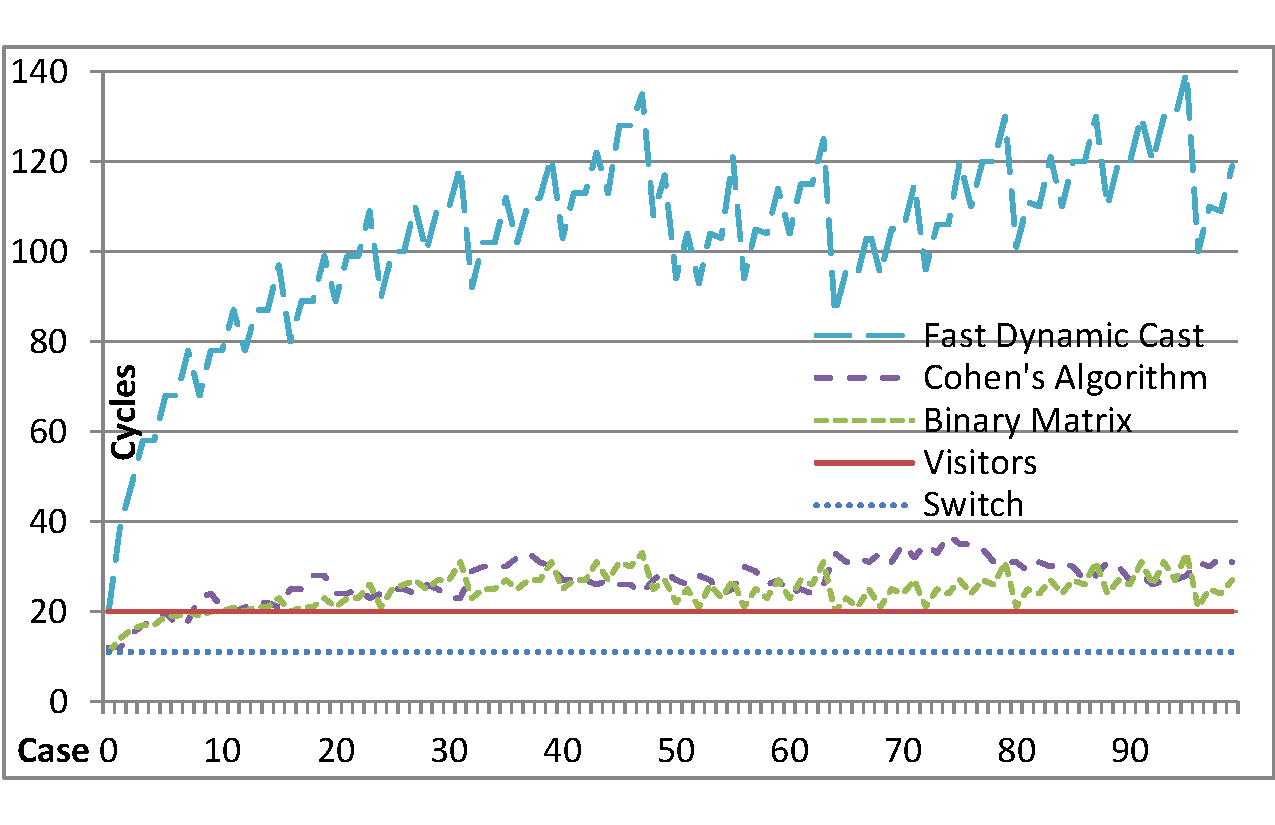
\includegraphics[width=0.47\textwidth]{DCast-vs-Visitors.pdf}
  \caption{Type switch based on constant-time subtype tests}
  \label{fig:DCastVis2}
\end{figure}

The chart in Figure~\ref{fig:DCastVis2} shows the number of cycles (Y-axis) each 
technique took to recognize an object of the dynamic type $i$ (X-axis). 
Despite known limitations, binary matrix and Cohen's algorithm are some of the 
fastest known type inclusion tests for single inheritance~\cite{Vitek97}. It 
is nonetheless easy to see that the logarithmic cost associated with the 
decision tree very quickly surpasses the constant overhead of double dispatch 
(20 cycles) present in the visitor design pattern or the jump-table 
implementation of the switch on all tags (11 cycles). We expect the cost of 
techniques capable of handling multiple inheritance to be even higher, especially 
those addressing casting between subobjects (e.g. fast dynamic cast). The edgy 
shape of timing results reflects the shape of the class hierarchy used for this 
experiment.
%We show in \textsection{sec:viscmp} that 
%our open solution is capable of delivering an amortized constant-time type 
%switching wi


\section{Type Switch}
\label{sec:copc}

While \Cpp{} does not have direct support for algebraic data types, they can be 
encoded with classes in a number of ways. One common such encoding is to 
introduce an abstract base class representing an algebraic data type with 
several derived classes representing variants. The variants can be 
discriminated with either run-time type information (referred to as 
\emph{polymorphic encoding}) or a unique tag inside a dedicated member of the 
common base class (referred to as \emph{tagged encoding}).

While \emph{Mach7} supports both encodings, it handles them differently to let 
the user choose between openness and efficiency. The type switch for tagged 
encoding (\textsection\ref{sec:cotc}) is simpler and more efficient for many typical use cases, however, 
making it open eradicates its performance advantages (\textsection\ref{sec:cmp}). 
%The difference in 
%performance is the price we pay for keeping the solution open. We describe pros 
%and cons of each approach in \textsection\ref{sec:cmp}.

%The core of the proposal relies on two key aspects of \Cpp{} implementations:
%\begin{enumerate}
%\item a constant-time access to the virtual table pointer embedded in an object of
%  dynamic class type;
%\item injectivity of the relation between an object's inheritance path
%  and the virtual table pointer extracted from that object.
%\end{enumerate}

\subsection{Attractive Non-Solution}
\label{sec:cotc}

%The memoization device outlined in \textsection\ref{sec:memdev} can, in principle, also be 
%applied to tagged classes. The dynamic cast will be replaced by a small 
%compile-time template meta-program that checks whether the class associated with 
%the given tag is derived from the target type of the case clause. If so, a static 
%cast can be used to obtain the offset.

%Despite its straightforwardness, we felt that it should be possible to do better 
%than the general solution, given that each class is already identified with a 
%dedicated constant known at compile time.

While Wirth' linked list encoding was considered slow for subtype testing it can 
be adopted for quite efficient type switching on a class hierarchy with no 
repeated inheritance. The idea is to combine the fast switching on closed 
algebraic datatypes with a loop that tries the tags of base classes when 
switching on derived tags fails.

%The nominal subtyping of C++ effectively gives every class multiple types. The 
%idea is thus to associate with the type not only its most-derived tag, but also 
%the list of tags of all its base classes. In a compiler implementation such a 
%list can be stored inside the virtual table of a class, while in our library 
%solution it is shared between all the instances with the same most-derived tag 
%in a less efficient global map, associating the tag to its tag list.

For simplicity of presentation we assume a pointer to array of tags be available 
directly through object's \code{taglist} data member. The array is of 
variable size, its first element is always the tag corresponding to the 
most-derived type of the object, while its end is marked with a dedicated 
\code{end_of_list} marker distinct from all the tags. The tags in between are 
topologically sorted according to the subtyping relation with incomparable 
siblings listed in \emph{local precedence order} -- the order of the direct base 
classes used in the class definition. The list resembles the \emph{class 
precedence list} of object-oriented descendants of Lisp (e.g. Dylan, Flavors, 
LOOPS, and CLOS) used there for \emph{linearization} of class hierarchies.
We also assume the tag-constant associated with a class 
\code{Di} be accessible through a static constant \code{Di::class_tag}. These 
simplifications are not essential and the library does not rely on any of these 
assumptions. Instead the user can retroactively narrate to the library the 
specific tag encoding used throught a trait-like classes.

A type switch below, built on top of a hierarchy of tagged classes, proceeds as 
a regular switch on the subject's tag. If the jump succeeds, we found an exact 
match; otherwise, we get into a default clause that obtains the next tag in the
list and jumps back to the beginning of the switch statement for a rematch:

\begin{lstlisting}
    size_t attempt = 0; 
    size_t tag = object->taglist[attempt];
ReMatch:
    switch (tag) {
    default:
        tag = object->taglist[++attempt];
        goto ReMatch;
    case end_of_list: 
        break;
    case D1::class_tag: 
        D1& match = static_cast<D1&>(*object); 
        s1; break;
        ...
    case Dn::class_tag: 
        Dn& match = static_cast<Dn&>(*object); 
        sn; break;
    }
\end{lstlisting}

\noindent
The above structure, which we call \emph{Tag Switch}, lets us dispatch to 
case clauses of the most-derived class with an overhead of initializing two 
local variables, compared to efficient switch used on algebraic data types. 
Dispatching to a case clause of a base class will take time roughly proportional 
to the distance between the matched base class and the most-derived class in the 
inheritance graph, thus the technique is not constant. When none of the base 
class tags were matched, we will necessarily reach the end\_of\_list marker in 
the list and exit the loop. As mentioned before, the default 
clause of the type switch can be implemented with a case clause on subject 
type's tag: \code{case S::class_tag:}

The efficiency of the above code crucially depends on the set of tags we match 
against be small and sequential to justify the use of jump table instead of 
decision tree to implement the switch. This is usually not a problem in closed 
hierarchies based on tag encoding since the user of the hierarchy hand-picks 
himself the tags. The use of static cast to obtain proper reference once the most 
specialized derived class has been established, however, essentially limits the use of 
this mechanism to single inheritance only. This of course only refers to the way target 
classes inherit from the subject type -- they can freely inherit other classes 
as long as they do not create repeated or virtual multiple inheritance of the 
subject type. Due to these assumptions, the technique is not open because it may 
violate independent extensibility. Moving away from these assumptions in order 
to make the technique more open (e.g. randomizing tags, using 
\code{dynamic_cast} etc.) will also eradicate its performance advantages.

\subsection{Open but Inefficient Solution}
\label{sec:poets}

Instead of starting with an efficient solution and trying to make it open, we 
start with an open solution and try to make it efficient. The following 
cascading-if statement implements the first-fit semantics for our type switch in 
a truly open fashion:

\begin{lstlisting}
if (T1* match=dynamic_cast<T1*>(subject)) {s1;} else
if (T2* match=dynamic_cast<T2*>(subject)) {s2;} else
...
if (Tn* match=dynamic_cast<Tn*>(subject)) {sn;}
\end{lstlisting}

\noindent
Its main drawback is performance: a typical implementation of 
\code{dynamic_cast} takes time proportional to the distance between base and 
derived classes in the inheritance tree. What is worse is that due to 
sequential order of tests, the time to uncover the type in the $i^{th}$ case 
clause will be proportional to $i$, while failure to match will take the longest. 
%This linear increase can be seen in the Figure~\ref{fig:DCastVis1}, where 
%the above cascading-if was applied to a flat hierarchy encoding an algebraic 
%data type with 100 variants. The same type-switching functionality implemented 
%with the visitor design pattern took only 28 cycles regardless of the 
%case.\footnote{Each case $i$ was timed multiple times, thus turning the experiment 
%into a repetitive benchmark described in \textsection\ref{sec:eval}. In a more
%realistic setting, represented by random and sequential benchmarks, the cost of 
%double dispatch was varying between 52 and 55 cycles.}
%This is more than 3 times faster than the 93 cycles it took to uncover even the 
%first case with \code{dynamic_cast}, while it took 22760 cycles to uncover the 
%last.
In a test involving a flat hierarchy of 100 variants, it took 93 cycles to 
discover the first type and 22760 to discover the last (with their linear combination 
for the types in between). %A visitor design pattern could 
%uncover any type in about 55 cycles, regardless of its position among the case 
%clauses, while a switch based on sequential tags could achieve the same in less 
%than 20 cycles. The idea is thus to combine the openness of the above structure 
%with the efficiency of a jump table on small sequential values.

Relying on \code{dynamic_cast} also makes an implicit semantic choice where we 
are no longer looking for the first/best-fitting type that is in subtyping 
relation, but for the first/best-fitting type to which a cast is possible from 
the source subobject (\textsection\ref{sec:specifics}).

%\begin{figure}[htbp]
%  \centering
%    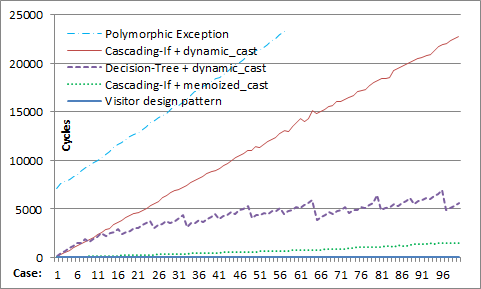
\includegraphics[width=0.47\textwidth]{DCast-vs-Visitors1.png}
%  \caption{Type switching based on na\"ive techniques}
%  \label{fig:DCastVis1}
%\end{figure}

%Seeing several solutions whose time increases with the position of the case 
%clause in the type switch, one may wonder how many such clauses a typical 
%program might have. A program dealing with abstract syntax trees in 
%Pivot~\cite{Pivot09} that we implemented using our pattern-matching library had 
%8 match statements with 5, 7, 8, 10, 15, 17, 30 and 63 case clauses, 
%respectively. With Pivot having the smallest number of node kinds among the 
%compiler frameworks we had a chance to work with, we expect a similar or larger 
%number of case clauses in other compiler applications.

%When the class hierarchy is not flat, the above cascading-if can be replaced 
%with a decision tree that tests base classes first and thus eliminates many of 
%the derived classes from consideration -- an approach used by Emir to deal with 
%type patterns in Scala~\cite[\textsection 4.2]{EmirThesis}. The intent is to 
%replace a sequence of independent dynamic casts between classes that are far 
%from each other in the hierarchy with nested dynamic casts between classes that 
%are close to each other. Another advantage is the possibility to fail early. 
%As can be seen from Figure~\ref{fig:DCastVis1} under ``Decision-Tree + 
%dynamic\_cast'', when applicable, the optimization can be very useful. The class
%hierarchy for this timing experiment formed a perfect binary tree with 
%classes number 2*N and 2*N+1 derived from a class with number N. The hierarchy 
%also explains the repetitive pattern of timings.
%
%Several authors had noted the relationship between exception handling and type 
%switching before~\cite{Glew99,ML2000}. Not surprisingly, the exception handling 
%mechanism of \Cpp{} can be abused to implement the first-fit semantics of a type 
%switch statement. The idea is to harness the fact that catch-handlers in \Cpp{} 
%essentially use first-fit semantics to decide which one is going to handle a 
%given exception. Unfortunately the approach is even slower than the use of 
%\code{dynamic_cast} and we only list it here for comparison.

\subsection{Memoization Device}
\label{sec:memdev}

Let us look at a slightly more general problem than type switching. Consider a 
generalization of the switch statement that takes predicates on a subject as its 
clauses and executes the first statement $s_i$ whose predicate is enabled: 

\begin{lstlisting}[keepspaces]
switch (x) { case P1(x): s1; ... case Pn(x): sn; }
\end{lstlisting}

\noindent
Assuming that predicates are \emph{functional} (i.e. do not involve any side 
effects), the next time we execute the switch with the same value $x$, the same 
predicate will be enabled first. We thus would like to avoid evaluating 
preceding predicates and jump to the statement it guards. In a way, we 
would like the switch to memoize the case enabled for a given $x$. 

The idea is to generate a simple cascading-if statement interleaved with jump 
targets and instructions that associate the original value with enabled target. 
The code before the statement looks up whether the association for a given value 
has already been established, and, if so, jumps directly to the target; otherwise, 
the sequential execution of the cascading-if is started. To ensure 
that the actual code associated with the predicates remains unaware of this 
optimization, the code preceding it after the target must re-establish any 
invariant guaranteed by sequential execution (\textsection\ref{sec:vtblmem}).

Described code can be easily produced in a compiler setting, but generating it in 
a library is a challenge. Inspired by Duff's Device~\cite{Duff}, 
we devised a construct that we call \emph{Memoization Device} doing just 
that in standard \Cpp{}:

\begin{lstlisting}
typedef decltype(x) T; // T is the type of subject x
static std::unordered_map<T,size_t> jump_targets;

switch (size_t& jump_to = jump_targets[x]) {
default: // entered when we have not seen x yet
    if (P1(x)) { jump_to = 1; case 1: s1; } else 
    if (P2(x)) { jump_to = 2; case 2: s2; } else
      ...
    if (Pn(x)) { jump_to = @$n$@; case @$n$@: sn; } else
                jump_to = @$n+1$@;
case @$n+1$@: // none of the predicates is true on x
}
\end{lstlisting}

\noindent
The static \code{jump_targets} hash table will be allocated upon first entry 
to the function. The map is initially empty and according to its logic, 
request for a key $x$ not yet in the map will allocate a 
new entry with its associated data default initialized (to 0 for \code{size_t}). Since 
there is no case label 0 in the switch, the default case will be taken, which, in 
turn, will initiate sequential execution of the interleaved cascading-if 
statement. Assignments to \code{jump_to} effectively establish association 
between value $x$ and corresponding predicate, since \code{jump_to} is a 
reference to \code{jump_targets[x]}. The last assignment records absence of 
enabled predicates for $x$.

To change the first-fit semantics of the above construct into \emph{sequential 
all-fit}, we remove the \code{else}-statements and rely on fall-through behavior of the 
switch. We make the assignments conditional to make sure only the first is recorded:

\begin{lstlisting}
if (Pi(x)) { if (jump_to == 0) jump_to = @$i$@; case @$i$@: si; }
\end{lstlisting}

\noindent
Note that the protocol that has to be maintained by this structure does not 
depend on the actual values of case labels. We only require them to be 
different and include a predefined default value. The default clause can be 
replaced with a case clause for the predefined value, however keeping the default  
clause results in a faster code. A more important performance consideration is to 
keep the values close to each other. Not following this rule might result in a 
compiler choosing a decision tree over a jump table implementation of the 
switch, which in our experience significantly degrades the performance.

The first-fit semantics is not an inherent property of the memoization device. 
Assuming that the conditions are either mutually exclusive or imply one another, we 
can build a decision tree based memoization device that will effectively have 
\emph{most-specific} semantics -- an analog of best-fit semantics in predicate 
dispatching~\cite{ErnstKC98}.

Imagine that the predicates with the numbers $2i$ and $2i+1$ are mutually exclusive and 
each imply the value of the predicate with number $i$ i.e.
$\forall i\forall x\in\bigcap_j\mathsf{Domain}(P_j).P_{2i+1}(x)\rightarrow P_i(x)\wedge P_{2i}(x)\rightarrow P_i(x)\wedge\neg(P_{2i+1}(x)\wedge P_{2i}(x))$ holds. 
An example of such predicates are class membership tests where the truth of 
testing membership in a derived class implies the truth of testing membership in 
its base class.

The following decision-tree based memoization device will execute the statement 
$s_i$ associated with the \emph{most-specific} predicate $P_i$ (i.e. the 
predicate that implies all other predicates true on $x$) that evaluates to true 
or will skip the entire statement if none of the predicates is true on $x$.

\begin{lstlisting}
switch (size_t& jump_to = jump_targets[x]) {
default:
    if (P1(x)) {
        if (P2(x)) {
            if (P4(x)) { jump_to = 4; case 4: s4; } else
            if (P5(x)) { jump_to = 5; case 5: s5; } 
            jump_to = 2; case 2: s2;
        } else
        if (P3(x)) {
            if (P6(x)) { jump_to = 6; case 6: s6; } else
            if (P7(x)) { jump_to = 7; case 7: s7; } 
            jump_to = 3; case 3: s3;
        }
        jump_to = 1; case 1: s1;
    } else { jump_to = 0; case 0: ; }
}
\end{lstlisting}

\noindent
Our library solution prefers the simpler cascading-if approach only because the 
necessary code structure can be laid out with macros. A compiler solution 
will use the decision-tree approach whenever possible to lower the cost of the 
first match from linear in case's number to logarithmic. % as seen in Figure\ref{fig:DCastVis1}.

%When the predicates do not satisfy the implication or mutual exclusion properties 
%mentioned above, a compiler of a language based on predicate dispatching would 
%typically issue an ambiguity error. Some languages might choose to resolve it 
%according to lexical or some other ordering. In any case, the presence of 
%ambiguities or their resolution has nothing to do with memoization device 
%itself. The latter only helps optimize the execution once a particular choice of 
%semantics has been made and code implementing it has been laid out.

The main advantage of the memoization device is that it can be built around 
almost any code, providing that we can re-establish the invariants, guaranteed 
by sequential execution. Its main disadvantage is the size of the hash table 
that grows proportionally to the number of different values seen. Fortunately, 
the values can often be grouped into equivalence classes that do not change the 
outcome of the predicates. The map can then associate the equivalence class of a 
value with a target instead of associating the value with it. 

In application to type switching, the idea is to use the memoization device to 
learn the outcomes of type inclusion tests (with \code{dynamic_cast} used as a 
predicate). The objects can be grouped into equivalence classes based on their 
most-derived type -- the outcome of each type inclusion test will be the same on 
all the objects of the same dynamic type. We can use the  
address of class' \code{type_info} object obtained in constant time with 
\code{typeid()} operator as a unique identifier of each most-derived type. 
Presence of multiple \code{type_info} objects for the same class, as is often 
the case when dynamic linking is involved, is not a problem, as it would 
effectively split a single equivalence class into multiple ones. 

This could have been a solution if we were only interested in class membership. 
More often than not, however, we will be interested in obtaining a reference to 
the target type of the subject and we saw in \textsection\ref{sec:specifics} 
that the cast between the source and target subobjects depends on 
the position of the source subobject in the most-derived type's subobject graph. 
We thus would like to have different equivalence classes per different 
subobjects. 
%, but there seems to be no easy way of identifying them given just an object descriptor.

\subsection{Virtual Table Pointers}
\label{sec:vtp}

%In this section we show that under certain conditions the compiler cannot share 
%the same virtual tables between different classes or their subobjects. This 
%allows us to use virtual table pointers to \emph{uniquely} identify the 
%subobjects within the most-derived class.

Figure~\ref{fig:objlayout} shows a typical object layout generated by a \Cpp{} 
compiler for class \code{D} from Figure~\ref{fig:inheritance}(1) under repeated 
(1) and virtual (2) inheritance of \code{A}. The layouts represent an encoding 
of the corresponding subobject graphs from Figures \ref{fig:inheritance}(2a) and 
\ref{fig:inheritance}(2b) respectively.

\begin{figure}[htbp]
  \centering
    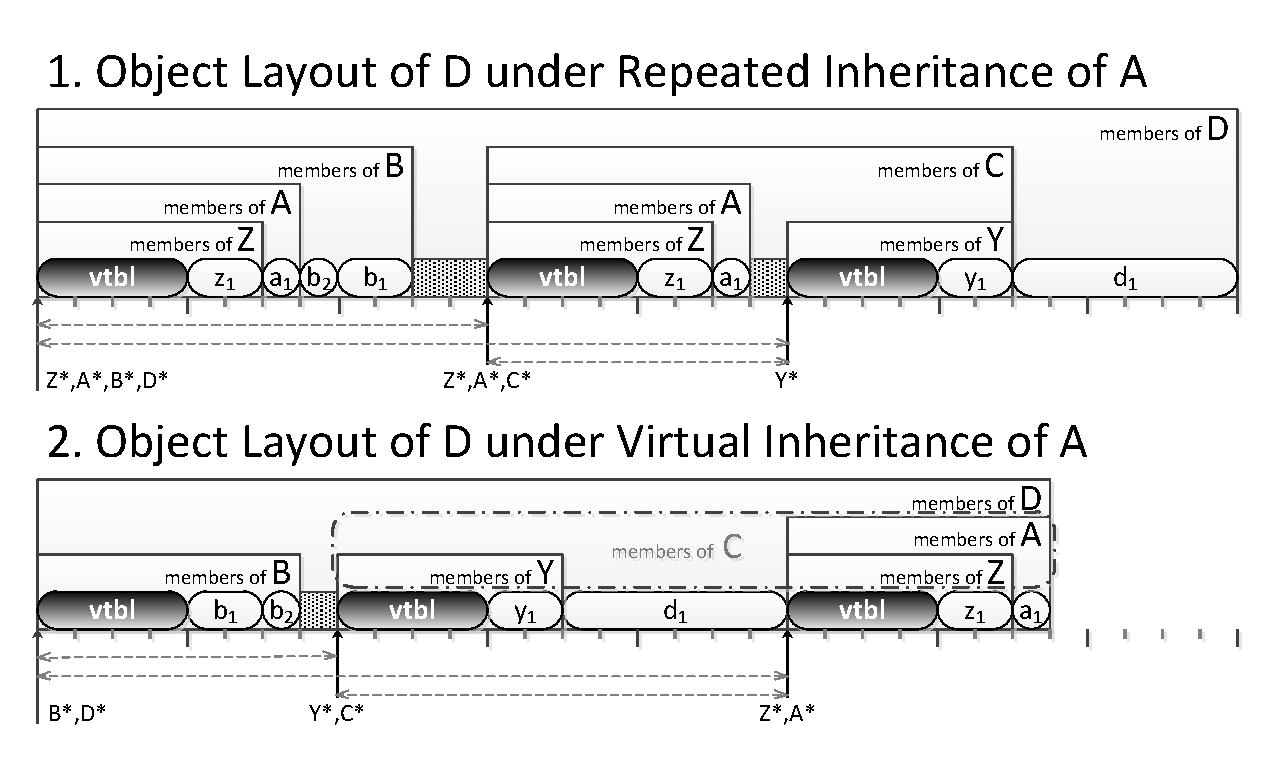
\includegraphics[width=0.47\textwidth]{obj-layout.pdf}
  \caption{Object Layout under Multiple Inheritance}
  \label{fig:objlayout}
\end{figure}

Due to extensibility of classes, the layout decisions for classes must be 
made independently of their derived classes -- a property of the \Cpp{} object 
model that we will refer to as \emph{layout independence}. In turn, the layout of derived   
classes must conform to the layout of its base classes relatively to the offset 
of the base class within derived. For example, the layout of \code{A} in 
\code{C} is exactly the same as the layout of \code{A} in \code{B} and is simply
the layout of \code{A}. Base classes inherited virtually do not contribute to 
the fixed layout because they are looked up indirectly at run-time, however, 
they are not exempt from the layout independence, since their lookup rules are 
agnostic of the concrete most-derived type.
%Because of this indirection, the use of virtual inheritance incures slight 
%overhead at run-time. 

Under non-virtual inheritance, members of the base class are typically laid out 
before the members of derived class resulting in the base class being at the 
same offset as the derived class itself. In our example, the offset of \code{A} 
in \code{B} under regular (non-virtual) inheritance of \code{A} is 0.
Under multiple inheritance, different base classes might be at different offsets 
in the most-derived class, which is why pointers of a given static type may be 
pointing to only certain subobjects in it. These positions are marked in the 
picture with vertical arrows decorated with the set of pointer types whose 
values may point into that position. Run-time conversions between such pointers 
represent casts between subobjects of the same most-derived type and may require 
adjustments to this-pointer (shown with dashed arrows) to maintain 
type safety.

A class that declares or inherits a virtual function is called a 
\emph{polymorphic class}. The \Cpp{} standard~\cite{C++11} does not prescribe any 
specific implementation technique for virtual function dispatch.
However, in practice, all \Cpp{} compilers use a strategy based on so-called
virtual function tables (or vtables for short) for efficient dispatch. 
The vtable is part of the reification of a polymorphic class type.  
\Cpp{} compilers embed a pointer to a vtable (vtbl-pointer for short) in every object of
polymorphic class type (and thus every subobject of that type inside other 
classes due to layout independence). CFront, the first \Cpp{} compiler, puts the 
vtbl-pointer 
at the end of an object. The so-called ``common vendor \Cpp{} ABI''\cite{C++ABI}, 
further referred to as \emph{\Cpp{} ABI} when not indicated otherwise, requires the 
vtbl-pointer to be at offset 0 of an object~\footnote{The following compilers 
are known to comply with the \Cpp{} ABI: GCC (3.x and up); Clang and llvm-g++; 
Linux versions of Intel and HP compilers, and compilers from ARM. See 
http://morpher.com/documentation/articles/abi/ for details.}. We do not have 
access to the unpublished Microsoft ABI, but we have experimental evidence that 
their \Cpp{} compiler also puts the vtbl-pointer at the start of an object.

While the exact offset of the vtbl-pointer within the (sub)object is not important 
for this discussion, because of layout independence every (sub)object of a 
polymorphic type \code{S} will have a vtbl-pointer at a predefined offset. 
Such offset may be different for different static types \code{S}, in which case 
the compiler will know at which offset in type \code{S} the vtbl-pointer is 
located, but it will be the same within any subobject of an effective type 
\code{S}. For a library implementation we assume presence of a function 
\code{template <typename S> intptr_t vtbl(const S* s);} 
that returns the address of the virtual table corresponding to the subobject 
pointed to by \code{s}. Such a function can be trivially implemented for the 
common \Cpp{} ABI, where the vtbl-pointer is always at offset 0:

\begin{lstlisting}
template <typename S> std::intptr_t vtbl(const S* s) {
    static_assert(std::is_polymorphic<S>::value, "error");
    return *reinterpret_cast<const std::intptr_t*>(s);
}
\end{lstlisting}

\noindent
Each of the \code{vtbl} fields shown in Figure~\ref{fig:objlayout} holds a 
vtbl-pointer referencing a group of virtual methods known in object's static 
type. Figure~\ref{fig:vtbl}(1) shows a typical layout of virtual function tables 
together with objects it points to for classes \code{B} and \code{D}.

\noindent
\begin{figure}[htbp]
  \centering
    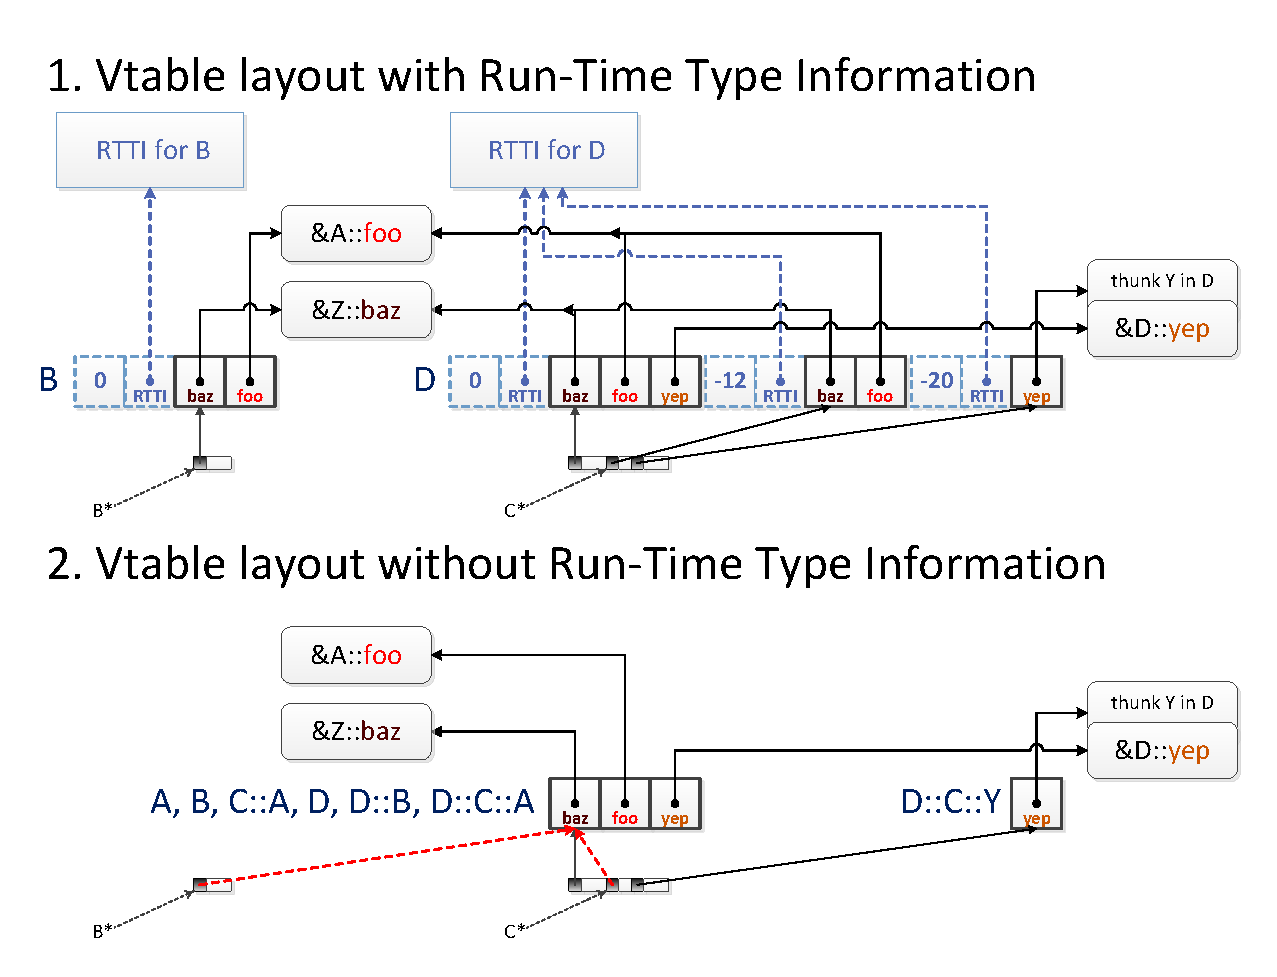
\includegraphics[width=0.49\textwidth]{v-table.pdf}
  \caption{VTable layout with and without RTTI}
  \label{fig:vtbl}
\end{figure}

Entries in the vtable to the right of the address pointed to by a vtbl-pointer 
represent pointers to functions, while entries to the left of it represent 
various additional fields like pointer to class' type information, offset to 
top, offsets to virtual base classes etc. In many implementations, this-pointer 
adjustments required to dispatch properly the call were stored in the vtable 
along with function pointers. Today most of the implementations prefer to use 
\emph{thunks} or \emph{trampolines} -- additional entry points to a function, 
that adjust this-pointer before transferring the control to the function, -- 
which was shown to be more efficient~\cite{Driesen96}. Thunks in general may 
only be needed when its virtual function is overridden. In such case, the 
overridden function may be called via pointer to base class or a pointer to 
derived class, which may not be at the same offset in the actual object.

The intuition behind our proposal is to use the values of vtbl-pointers stored 
inside the object to identify uniquely the subobject in it. There are several 
problems with the approach, however. First, the same vtbl-pointer is 
usually shared by multiple subobjects when one of them contains the other. For 
example, the first vtbl-pointer in Figure~\ref{fig:objlayout}(1) will be shared 
by objects of static type \code{Z*}, \code{A*}, \code{B*} and \code{D*}. This is 
not a problem for our purpose, because the subobjects of these types will be at 
the same offset in the most-derived object. Secondly, and more importantly, 
however, there are legitimate optimizations that let the compiler share the same 
vtable among multiple subobjects of often-unrelated types.

Generation of the \emph{Run-Time Type Information} (or RTTI for short) can 
typically be disabled with a compiler switch and the Figure~\ref{fig:vtbl}(2) 
shows the same vtable layouts once the RTTI has been disabled. Since neither 
\code{baz} nor \code{foo} were overridden, the prefix of the vtable for the 
\code{C} subobject in \code{D} is exactly the same as the vtable for its 
\code{B} subobject, the \code{A} subobject of \code{C} or the entire vtable of 
\code{A} and \code{B} classes. Such layout, for example, is produced by 
Microsoft Visual \Cpp{} 11 when the command-line option \code{/GR-} is specified. 
Visual \Cpp{} compiler has been known to unify code identical on binary level, 
which in some cases may result in sharing of the same vtable between unrelated 
classes (e.g., when virtual functions are empty).

%\Cpp{} supports multiple-inheritance of two kinds: repeated and virtual (shared). 
%\emph{Repeated inheritance} creates multiple independent subobjects of the same 
%type within the most-derived type. \emph{Virtual inheritance} creates only one 
%shared subobject, regardless of the inheritance paths. Consequently,
%it is not sufficient to talk only about the 
%static and dynamic types of an object -- one has to talk about a 
%\emph{subobject} of a certain static type accessible through a given inheritance 
%path within a dynamic type. 

We now would like to show more formally that in the presence of RTTI, a \Cpp{} ABI 
compliant implementation would always have all the vtbl-pointers different. To do 
so, we need a closer look at the notion of subobject, which has been formalized 
before~\cite{RF95,WNST06,RDL11}. We follow here the presentation of Ramamanandro 
et al~\cite{RDL11}.

\subsection{Subobjects}
\label{sec:subobj}

We assume a program $\mathfrak{P}$ is represented by its class table, which can be 
queried for inheritance relations between classes. All subsequent definitions 
are implicitly parameterized over a given program $\mathfrak{P}$. 
A class $B$ is a \emph{direct repeated base class} of  
$D$ if $B$ is mentioned in the list of base classes of $D$ without the 
\code{virtual} keyword ($D \prec_R B$). Similarly, a class $B$ is a \emph{direct 
shared base class} of $D$ if $B$ is mentioned in the list of base classes of $D$ 
with the \code{virtual} keyword ($D \prec_S B$). A reflexive transitive closure 
of these relationships $\preceq^*=(\prec_R \cup \prec_S)^*$ defines the 
\emph{subtyping} relation on types of program $\mathfrak{P}$.
A base class \emph{subobject} of a given \emph{complete object} is represented by a pair 
$\sigma = (h,l)$ with $h \in \{\mathsf{Repeated},\mathsf{Shared}\}$ representing the 
kind of inheritance (single inheritance is $\mathsf{Repeated}$ with one base class) and $l$ 
representing the path in a non-virtual inheritance graph.
A judgment of the form $\mathfrak{P}\vdash C\leftY\sigma\rightY A$ states that 
in a program $\mathfrak{P}$, $\sigma$ designates a subobject of static type $A$ 
within the most-derived object of type $C$. Omitting the context $\mathfrak{P}$: 

\begin{mathpar}
\inferrule
{C \prec_S B \\ B\leftY(h,l)\rightY A}
{C\leftY(\mathsf{Shared},l)\rightY A}

\inferrule
{}
{C\leftY(\mathsf{Repeated},C::\epsilon)\rightY C}

\inferrule
{C \prec_R B \\ B\leftY(\mathsf{Repeated},l)\rightY A}
{C\leftY(\mathsf{Repeated},C::l)\rightY A}
\end{mathpar}

\noindent
$\epsilon$ indicates an empty path, but we will generally omit it in writing 
when understood from the context. In case of repeated inheritance in 
Figure~\ref{fig:inheritance}(1), an object of the most-derived class \code{D} 
will have the following $\mathsf{Repeated}$ subobjects:
\code{D::C::Y}, 
\code{D::B::A::Z}, 
\code{D::C::A::Z}, 
\code{D::B::A}, 
\code{D::C::A}, 
\code{D::B}, 
\code{D::C}, 
\code{D}.
Similarly, in case of virtual inheritance in the same example, an object of the 
most-derived class \code{D} will have the following $\mathsf{Repeated}$ subobjects:
\code{D::C::Y}, 
\code{D::B}, 
\code{D::C}, 
\code{D}
as well as the following $\mathsf{Shared}$ subobjects: 
\code{D::A::Z}, 
\code{D::Z}, 
\code{D::A}. See Figure~\ref{fig:inheritance} for illustration.

It is easy to show by structural induction on the above definition, that 
$C\leftY\sigma\rightY A \implies \sigma=(h,C::l_1) \wedge \sigma=(h,l_2::A::\epsilon)$, 
which simply means that any path to a subobject of static type $A$ within the 
most-derived object of type $C$ starts with $C$ and ends with $A$. This 
observation shows that $\sigma_\bot = (\mathsf{Shared},\epsilon)$ does not 
represent a valid subobject. If $\Sigma_\mathfrak{P}$ is the domain of all subobjects in 
the program $\mathfrak{P}$ extended with $\sigma_\bot$, then a \emph{cast} operation can be 
understood as a function $\delta : \Sigma_\mathfrak{P} \rightarrow \Sigma_\mathfrak{P}$. We use 
$\sigma_\bot$ to indicate an impossibility of a cast. The fact that $\delta$ is 
defined on subobjects as opposed to actual run-time values reflects the 
non-coercive nature of the operation -- i.e. the underlain value remains the 
same. Any implementation of such a function must thus satisfy the following 
condition:
\begin{eqnarray*}
C \leftY\sigma_1\rightY A \wedge \delta(\sigma_1) = \sigma_2 \implies C \leftY\sigma_2\rightY B
\end{eqnarray*}
\noindent
i.e. the most-derived type of the value does not change during casting, only the way 
we reference it does. Following the definitions from 
\textsection\ref{sec:specifics}, $A$ is the \emph{source type} and $\sigma_1$ is 
the \emph{source subobject} of the cast, while $B$ is the \emph{target type} and 
$\sigma_2$ is the \emph{target subobject} of it. The type $C$ is the 
most-derived type of the value being casted. The \Cpp{} semantics states more 
requirements to the implementation of $\delta$: e.g. 
$\delta(\sigma_\bot) = \sigma_\bot$ etc. but their precise modeling is out of 
scope of this discussion. We would only like to point out here that since 
the result of the cast does not depend on the actual value and only on the 
source subobject and the target type, we can memoize the outcome of a cast on 
one instance in order to apply its results to another.

%Figure~\ref{fig:objlayout}(1)
%$Z\leftY(\mathsf{Repeated},      [Z])\rightY Z$,
%$A\leftY(\mathsf{Repeated},    [A,Z])\rightY Z$,
%$B\leftY(\mathsf{Repeated},  [B,A,Z])\rightY Z$,
%$D\leftY(\mathsf{Repeated},[D,B,A,Z])\rightY Z$,
%$C\leftY(\mathsf{Repeated},  [C,A,Z])\rightY Z$,
%$D\leftY(\mathsf{Repeated},[D,C,A,Z])\rightY Z$,
%$Y\leftY(\mathsf{Repeated},      [Y])\rightY Y$,  
%$C\leftY(\mathsf{Repeated},    [C,Y])\rightY Y$,
%$D\leftY(\mathsf{Repeated},  [D,C,Y])\rightY Y$,
%$A\leftY(\mathsf{Repeated},      [A])\rightY A$, 
%$B\leftY(\mathsf{Repeated},    [B,A])\rightY A$,
%$D\leftY(\mathsf{Repeated},  [D,B,A])\rightY A$,
%$C\leftY(\mathsf{Repeated},    [C,A])\rightY A$,
%$D\leftY(\mathsf{Repeated},  [D,C,A])\rightY A$,
%$B\leftY(\mathsf{Repeated},      [B])\rightY B$,
%$D\leftY(\mathsf{Repeated},    [D,B])\rightY B$,
%$C\leftY(\mathsf{Repeated},      [C])\rightY C$,
%$D\leftY(\mathsf{Repeated},    [D,C])\rightY C$,
%$D\leftY(\mathsf{Repeated},      [D])\rightY D$,
%
%Figure~\ref{fig:objlayout}(2)
%$Z\leftY(\mathsf{Repeated},      [Z])\rightY Z$,
%$A\leftY(\mathsf{Repeated},    [A,Z])\rightY Z$,
%$B\leftY(\mathsf{Shared},    [B,A,Z])\rightY Z$,
%$C\leftY(\mathsf{Shared},    [C,A,Z])\rightY Z$,
%$D\leftY(\mathsf{Shared},    [D,A,Z])\rightY Z$,
%$D\leftY(\mathsf{Shared},      [D,Z])\rightY Z$,
%$Y\leftY(\mathsf{Repeated},      [Y])\rightY Y$,  
%$C\leftY(\mathsf{Repeated},    [C,Y])\rightY Y$,
%$D\leftY(\mathsf{Repeated},  [D,C,Y])\rightY Y$,
%$A\leftY(\mathsf{Repeated},      [A])\rightY A$, 
%$B\leftY(\mathsf{Shared},      [B,A])\rightY A$,
%$C\leftY(\mathsf{Shared},      [C,A])\rightY A$,
%$D\leftY(\mathsf{Shared},      [D,A])\rightY A$,
%$B\leftY(\mathsf{Repeated},      [B])\rightY B$,
%$D\leftY(\mathsf{Repeated},    [D,B])\rightY B$,
%$C\leftY(\mathsf{Repeated},      [C])\rightY C$,
%$D\leftY(\mathsf{Repeated},    [D,C])\rightY C$,
%$D\leftY(\mathsf{Repeated},      [D])\rightY D$,

\subsection{Uniqueness of vtbl-pointers under the \Cpp{} ABI}
\label{sec:uniq}

%A class that declares or inherits a virtual function is called a 
%\emph{polymorphic class}~\cite[\textsection 10.3]{C++11}.  We say that
%a class is \emph{dynamic} \cite{C++ABI} if it requires a virtual table pointer 
%(because it or its bases have one or more virtual member functions or
%virtual base classes). 
%A \emph{virtual table pointer} (vtbl-pointer)
%is a data-member of an object pointing to the object's dynamic type vtable.
%In addition to dispatching virtual function calls, it is used to access
%virtual base class subobjects, and to 
%access \emph{RunTime Type Identification} (RTTI) data.
%An object of a class
%type with multiple inheritance may contain several vtbl-pointers
%(included in its subobjects). We assume that for every expression of
%static type \code{T} (a dynamic class type), a \Cpp{} compiler provides
%access to the vtbl-pointer of the (sub)object designated by that 
%expression (or at least documents the position of that
%pointer within an object). For the common vendor \Cpp{} ABI, we can state:
%\begin{lemma}
%  In an object layout that adheres to the ``common vendor \Cpp{} ABI'', 
%  an object of a polymorphic class always has a virtual table pointer
%  at offset 0.
%\label{lem:vtbl}
%\end{lemma}

%\noindent
%With no further assumption, we cannot use a vtable to uniquely identify
%its dynamic type or those of its subobjects. The reason is that a popular 
%compression technique is to share compiler-generated data, and not exclusively
%between subobjects in the class hierarchy.
%Use of such optimization will violate the 
%uniqueness of vtbl-pointers; however, we show below that in the presense of 
%runtime type identification information (RTTI), we have a form of injectivity
%that is sufficient for our needs.
Given a reference \code{a} to polymorphic type \code{A} that points to a subobject 
$\sigma$ of the most-derived type \code{C} (i.e. $C\leftY\sigma\rightY A$ is 
true), we will use the traditional field-access notion \code{a.vtbl} to refer to 
the virtual table of that subobject. The exact structure of the virtual table as 
mandated by the common vendor \Cpp{} ABI is immaterial for this discussion, but we 
mention a few fields that are important for the reasoning~\cite[\textsection 2.5.2]{C++ABI}:

\begin{itemize}
\setlength{\itemsep}{0pt}
\setlength{\parskip}{0pt}
\item \code{rtti(a.vtbl)}: the \emph{typeinfo pointer} points to the typeinfo 
      object used for RTTI. It is always present and is shown as the first field 
      to the left of any vtbl-pointer in Figure~\ref{fig:vtbl}(1).
\item \code{off2top(a.vtbl)}: the \emph{offset to top} holds the displacement to 
      the top of the object from the location within the object of the 
      vtbl-pointer that addresses this virtual table. It is always present and 
      is shown as the second field to the left of any vtbl-pointer in 
      Figure~\ref{fig:vtbl}(1). The numeric value shown indicates the actual 
      offset based on the object layout from Figure~\ref{fig:objlayout}(1).
\item \code{vbase(a.vtbl)}: \emph{Virtual Base (vbase) offsets} are used to access 
      the virtual bases of an object. Such an entry is required for each virtual 
      base class. None is shown in our example in Figure~\ref{fig:vtbl}(1) 
      since it discusses repeated inheritance, but they will occupy further 
      entries to the left of the vtbl-pointer, when present.
\end{itemize}

\noindent
We also use the notation $\mathit{offset}(\sigma)$ to refer to the offset of a 
given subobject $\sigma$ within $C$, known by the compiler.

\begin{theorem}
In an object layout that adheres to the common vendor \Cpp{} ABI with enabled RTTI, 
equality of vtbl-pointers of two objects of the same static type implies that 
they both belong to subobjects with the same inheritance path in the same most-derived class.

\noindent
$\forall a_1, a_2 : A\ |\ a_1\in C_1\leftY\sigma_1\rightY A \wedge a_2\in C_2\leftY\sigma_2\rightY A $ \\ 
$a_1.\textit{vtbl} = a_2.\textit{vtbl} \Rightarrow C_1 = C_2 \wedge \sigma_1 = \sigma_2$
\label{thm:vtbl}
\end{theorem}
\begin{proof}
Let us assume first $a_1.\textit{vtbl} = a_2.\textit{vtbl}$ but $C_1 \neq C_2$. In this case we 
have \code{rtti}$(a_1.\textit{vtbl}) = $\code{rtti}$(a_2.\textit{vtbl})$. By definition 
\code{rtti}$(a_1.\textit{vtbl}) = C_1$ while \code{rtti}$(a_2.\textit{vtbl}) = C_2$, which 
contradicts that $C_1 \neq C_2$. Thus $C_1 = C_2 = C$.

Let us assume now that $a_1.\textit{vtbl} = a_2.\textit{vtbl}$ but $\sigma_1 \neq \sigma_2$. 
Let $\sigma_1=(h_1,l_1),\sigma_2=(h_2,l_2)$ 

If $h_1 \neq h_2$ then one of them refers to a virtual base while the other to a 
repeated one. Assuming $h_1$ refers to a virtual base, \code{vbase}$(a_1.\textit{vtbl})$ 
has to be defined inside the vtable according to the ABI, while 
\code{vbase}$(a_2.\textit{vtbl})$ -- should not. This would contradict again that both 
$vtbl$ refer to the same virtual table.

We thus have $h_1 = h_2 = h$. If $h = \mathsf{Shared}$ then there is only one path to 
such $A$ in $C$, which would contradict $\sigma_1 \neq \sigma_2$. 
If $h = \mathsf{Repeated}$ then we must have that $l_1 \neq l_2$. In this case let $k$ be 
the first position in which they differ: 
$\forall j<k.l_1^j=l_2^j \wedge l_1^k\neq l_2^k$. Since our class $A$ is a base 
class for classes $l_1^k$ and $l_2^k$, both of which are in turn base classes of 
$C$, the object identity requirement of \Cpp{} requires that the relevant subobjects 
of type $A$ have different offsets within class $C$: 
$\mathit{offset}(\sigma_1)\neq \mathit{offset}(\sigma_2)$ However 
$\mathit{offset}(\sigma_1)=$\code{off2top}$(a_1.\textit{vtbl})=$\code{off2top}$(a_2.\textit{vtbl})=\mathit{offset}(\sigma_2)$ 
since $a_1.\textit{vtbl} = a_2.\textit{vtbl}$, which contradicts that the offsets are different.
\end{proof}

\noindent
Conjecture in the other direction is not true in general as there may be 
duplicate vtables for the same type present at run-time. This happens in 
many \Cpp{} implementations in the presence of \emph{Dynamically Linked Libraries} 
(or DLLs for short) as the same class compiled into executable and DLL it loads 
may have identical vtables inside the executable's and DLL's binaries.

Note also that we require both static types to be the same. Dropping this 
requirement and saying that equality of vtbl-pointers also implies equality of 
the static types is not true in general because a derived class can share the 
vtbl-pointer with its primary base class. The theorem can be reformulated, 
however, stating that one subobject will necessarily have to containe the other, but that would require bringing in the formalism for subobject 
containment~\cite{WNST06}. The current formulation is sufficient for our 
purposes.

%\begin{corollary}
%In an object layout that adheres to the common vendor \Cpp{} ABI with enabled RTTI, 
%the offset between two same subobjects of two different objects of the same 
%most-derived type is the same.
%$\forall c_1, c_2 : C\ |\ c_1,c_2 \in C\leftY\sigma_1\rightY C $ \\ 
%$a_1.\textit{vtbl} = a_2.\textit{vtbl} \Rightarrow C_1 = C_2 \wedge \sigma_1 = \sigma_2$
%
%
%Results of \code{dynamic_cast} can be reapplied to a different instance from 
%within the same subobject. 
%
%$\forall A,B \forall a_1, a_2 : A\ |\ a_1.\textit{vtbl} = a_2.\textit{vtbl} \Rightarrow$ \\
%\code{dynamic_cast<B>}$(a_1).\textit{vtbl}_j = $\code{dynamic_cast<B>}$(a_2).\textit{vtbl}_j \vee$ \\
%\code{dynamic_cast<B>}$(a_1)$ throws $\wedge$ \code{dynamic_cast<B>}$(a_2)$ throws.
%\label{crl:vtbl}
%\end{corollary}

%\noindent
During construction and deconstruction of 
an object, the value of a given vtbl-pointer may change. In particular, 
that value will reflect the fact that the most-derived type of the object is the type of its 
fully constructed part only. This, however, does not affect our reasoning, as during 
such transition we also treat the object to have the type of its fully 
constructed base only. Such interpretation is in line with the \Cpp{} semantics for 
virtual function calls and the use of RTTI during construction and destruction of an 
object. Once the complete object is fully constructed, the value of the 
vtbl-pointer will remain the same for the lifetime of the object.

\subsection{Vtable Pointer Memoization}
\label{sec:vtblmem}

%The memoization device can almost immediately be used for multi-way type testing by 
%using \code{dynamic_cast<Ti>} as a predicate $P_i$. This cannot be considered a 
%type switching solution, however, as one would expect to also have a reference 
%to the uncovered type. Using a \code{static_cast<Ti>} upon successful type test 
%would have been a solution if we did not have multiple inheritance. It certainly 
%can be used as such in languages with only single inheritance. For the fully 
%functional \Cpp{} solution, we combine the memoization device with the properties 
%of virtual table pointers into a \emph{Vtable Pointer Memoization} technique.

The \Cpp{} standard implies that information about types be available at run time 
for three distinct purposes~\cite[\textsection 2.9.1]{C++ABI}:

\begin{itemize}
\setlength{\itemsep}{0pt}
\setlength{\parskip}{0pt}
\item to support the \code{typeid} operator,
\item to match an exception handler with a thrown object, and
\item to implement the \code{dynamic_cast} operator.
\end{itemize}

\noindent
and if any of these facilities are used in a program that was compiled with 
disabled RTTI, the compiler shall emit a warning. Some 
compilers (e.g. Visual \Cpp{}) additionally let a library check presence of RTTI 
through a predefined macro, thus letting it report an error if its dependence on 
RTTI cannot be satisfied. Since our solution depends on \code{dynamic_cast}% to perform casts at run-time
, according to the third requirement we implicitly rely on the presence of RTTI and thus 
fall into the setting that guarantees the preconditions of Theorem~\ref{thm:vtbl}.
Besides, all the objects that will be coming through a particular type switch will 
have the same static type, and thus the theorem guarantees that different vtbl-pointers 
will correspond to different subobjects. The idea is thus to group them 
accordingly to the value of their vtbl-pointer and associate both jump target 
and the required offset through the memoization device:

\begin{lstlisting}
typedef pair<ptrdiff_t,size_t> target_info; //(offs,targ)
static unordered_map<intptr_t, target_info> jump_targets;
      auto*  sptr = &x; // name to access subject
const void*  tptr; 
target_info& info = jump_targets[vtbl(sptr)];
switch (info.second) {{ default: 
\end{lstlisting}

\noindent
The code for the $i^{th}$ case now evaluates the required offset on the first 
entry and associates it and the target with the vtbl-pointer of the subject.
The call to \code{adjust_ptr<Ti>} re-establishes the invariant that 
\code{match} is a reference to type \code{Ti} of the subject \code{x}.
%The condition of the inner if-statement is only needed to implement the 
%sequential all-fit semantics and can be removed when fall-through behavior is 
%not required.

\begin{lstlisting}
  if (tptr = dynamic_cast<const Ti *>(sptr)) {
    if (info.second == 0) { // supports fall-through
      info.first  = intptr_t(tptr)-intptr_t(sptr); // offset
      info.second = @$i$@; // jump target
    }
  case @$i$@: // @$i$@ is a constant - clause's position in switch
    auto match = adjust_ptr<Ti>(sptr,info.first);
    si;
  }
\end{lstlisting}

\noindent
%The use of dynamic cast makes a huge difference in comparison to the use of 
%static cast we dismissed above. First of all the \Cpp{} type system is much more 
%restrictive about the static cast and many cases where it is not allowed can 
%still be handled by dynamic cast. Examples of these include downcasting from an 
%ambiguous base class or crosscasting between unrelated base classes.
%
%An important benefit we get from this optimization is that the number of values 
%stored in the hash table is on the order $O(|A|)$, where $A$ represents the 
%static type of an object, while $|A|$ represents the number of classes directly 
%or indirectly derived from $A$. The linear coefficient of the big-o notation 
%reflects possibly multiple vtbl-pointers in derived classes due to multiple 
%inheritance.

\noindent
Class \code{std::unordered_map} provides amortized constant time access on 
average and linear in the number of elements in the worst case. We show in the 
next section that most of the time we will be bypassing traditional access to 
its elements. We need this extra optimization because, as-is, the type switch is 
still about 50\% slower than the visitor design pattern.\footnote{We are using 
speedups throughout the paper when comparing performance, so ``X is 42\% faster 
than Y'' or equally ``Y is 42\% slower than X'' means that Y's execution time is 
1.42 times X's execution time.}

%Note that we can apply the reasoning of \textsection\ref{sec:memdev} and change 
%the first-fit semantics of the resulting match statement into a best-fit 
%semantics simply by changing the underlying cascading-if structure with decision 
%tree. A compiler implementation of a type switch based on Vtable Pointer 
%Memoization will certainly take advantage of this optimization to cut down the 
%cost of the first run on a given vtbl-pointer, when the actual memoization happens.

Looking back at example from \textsection\ref{sec:intro} and allowing for few 
unimportant omissions, the first code snippet corresponds to what macro 
\code{Match(x)} is expanded to given a subject expression \code{x}. In order to 
see what \code{Case(Ti)} is expanded to, the second snippet has to be split on 
the line containing \code{si;} (excluding \code{si;} itself, which comes from 
source) and the second part (i.e. \} here) moved in front of the first one. The 
macro thus closes the scope of the previous case-clause, before starting the new 
one. \code{Case}'s expansion only relies on names introduced by \code{Match(x)}, 
its argument \code{Ti} and a constant $i$, which can be generated from 
\code{__LINE__} or better \code{__COUNTER__} macro when the later one is 
supported by the compiler. The \code{EndMatch} macro simply closes the scopes 
(i.e. \}\} here). We refer the reader to consult the library source code for 
further details.

%\subsubsection{Structure of Virtual Table Pointers}
%\label{sec:sovtp}

\subsection{Minimization of Conflicts}
\label{sec:moc}

Virtual table pointers are not constant values and are not even guaranteed to be 
the same between different runs of the application, because techniques like 
\emph{address space layout randomization} or \emph{rebasing} of the module are 
likely to change them. The relative distance between them will remain the same 
however, as long as they come from the same module.

Knowing that vtbl-pointers point into an array of function pointers, we should 
expect them to be aligned accordingly and thus have a few lowest bits as zero. 
Moreover, since many derived classes do not introduce new virtual functions, 
the size of their virtual tables remains the same. When allocated sequentially 
in memory, we can expect a certain number of lowest bits in the vtbl-pointers 
pointing to them to be the same.
These assumptions, supported by actual observations, made virtual table 
pointers of classes related by inheritance ideally suitable for hashing -- the 
values obtained by throwing away the common bits on the right were compactly 
distributed in small disjoint ranges (\textsection\ref{sec:hierarchies}). We use 
them to address a cache built on top of the hash table in order to eliminate a 
hash table lookup in most of the cases.

Let $\Xi$ be the domain of integral representations of pointers. Given a cache 
with $2^k$ entries, we use a family of hash functions $H_{kl} : \Xi \rightarrow [0..2^k-1]$ 
defined as $H_{kl}(v)=v/2^l \mod 2^k$ to index the cache, where $l \in [0..32]$ 
(assuming 32 bit addresses) is a parameter modeling the number of common bits on 
the right. Division and modulo are implemented with bit operations since 
denominator in each case is a power of 2, which in turn explains the choice of 
the cache size.

Given a hash function $H_{kl}$, pointers $v'$ and $v''$ are said to be in 
\emph{conflict} when $H_{kl}(v')=H_{kl}(v'')$. For a given set of pointers 
$V \in 2^{\Xi}$, we can always find such $k$ and $l$ that $H_{kl}$ will render no  
conflicts between its elements, however the required cache size $2^k$ can be too 
large to justify the use of memory. The value $K$ such that $2^{K-1} < |V| \leq 2^K$ 
is the smallest value of $k$ under which absence of conflicts is still possible. 
We thus allow $k$ to vary only in range $[K,K+1]$ to ensure that the cache size 
is never more than 4 times bigger than the minimum required cache size.

Given a set $V = \{v_1, ... , v_n\}$, we would like to find a pair of parameters 
$(k,l)$ such that $H_{kl}$ will render the least number of conflicts on the 
elements of $V$. Since for a fixed set $V$, parameters $k$ and $l$ vary in a 
finite range, we can always find the optimal $(k,l)$ by trying all the
combinations. Let $H_{kl}^V : V \rightarrow [0..2^k-1]$ be the hash function 
corresponding to such optimal $(k,l)$ for the set $V$. 

In our setting, set $V$ represents the set of vtbl-pointers coming through a 
particular type switch. While the exact values of these pointers are not known 
until run-time, their offset from the module's base address is. This is generally 
sufficient to estimate optimal $k$ and $l$ in a compiler setting. In the library 
setting, we recompute them after a given number of actual collisions in cache.

When $H_{kl}^V$ is injective (renders 0 conflicts on $V$), the frequency of any 
given vtbl-pointer $v_i$ coming through the type switch does not affect the 
overall performance of the switch. However when $H_{kl}^V$ is not injective, we 
would prefer the conflict to happen on less frequent vtbl-pointers.
Given a probability $p(v_i)$ of each vtbl-pointer $v_i \in V$ we can compute the 
probability of conflict rendered by a given $H_{kl}$:

\begin{eqnarray*}
p_{kl}(V)=\sum\limits_{j=0}^{2^k-1}(\sum\limits_{v_{i} \in V^j_{kl}}p(v_i))(1-\frac{\sum\limits_{v_i \in V^j_{kl}}p(v_i)^2}{(\sum\limits_{v_{i} \in V^j_{kl}}p(v_i))^2})
\end{eqnarray*}

\noindent 
where $V^j_{kl}=\{v \in V | H_{kl}(v)=j\}$. In this case, the optimal hash 
function $H_{kl}^V$ can similarly be defined as $H_{kl}$ that minimizes the 
above probability of conflict on $V$.

Probabilities $p(v_i)$ can be estimated in a compiler setting through profiling, 
while in a library setting we let the user enable tracing of frequencies of 
each vtbl-pointer. This introduces an overhead of an increment into the critical 
path of execution, and according to our tests degrades the performance by 1-2\%. 
This should not be a problem as long as the overall performance gains from 
smaller probability of a conflicts happening at run time. Unfortunately, in our 
tests the significant drop in the number of actual collisions was not reflected 
in a noticeable decrease in execution time, which is why we do not enable 
frequency tracing by default. As we will see in \textsection\ref{sec:hierarchies}, 
this was happening because the hash function $H_{kl}^V$ renders no conflicts on 
vtbl-pointers in most of the cases and the few collisions we were getting before 
inferring the optimal $k$ and $l$ even in non-frequency based caching where 
incomparably smaller than the number of successful cache hits.

Assuming the uniform distribution of $v_i$ in $V$ and substituting the probability 
$p(v_i)=\frac{1}{n}$, where $n=|V|$, into the above formula we get:

\begin{eqnarray*}
p_{kl}(V)=\sum\limits_{j=0}^{2^k-1}[|V^j_{kl}| \neq 0]\frac{|V^j_{kl}|-1}{n}
\end{eqnarray*}

\noindent
We use the Iverson bracket $[\pi]$ here to refer to the outcome of a predicate $\pi$ as numbers $0$ or $1$.
The value $|V^j_{kl}|$ represents the number of vtbl-pointers $v_i \in V$ that are mapped to the same location $j$ in cache with $H_{kl}^V$. Only 
one such vtbl-pointer will actually be present in that cache location at any given 
time, which is why the value $|V^j_{kl}|-1$ represents the number of ``extra'' 
pointers mapped into the entry $j$ on which a collision will happen. The overall 
probability of conflict thus only depends on the total number of these ``extra'' 
or conflicting vtbl-pointers. The $H_{kl}^V$ obtained by minimization of 
probability of conflict under uniform distribution of $v_i$ in $V$ is thus the 
same as original $H_{kl}^V$ that was minimizing the number of conflicts. An 
important observation here is that since the exact location of these ``extra'' 
vtbl-pointers is not important and only the total number $m$ is, the probability 
of conflict under uniform distribution of $v_i$ in $V$ is always going to be of 
discrete form $\frac{m}{n}$, where $0 \le m < n$.

%Depending on the number of actual collisions that happen in the cache, our 
%vtable pointer memoization technique can come close to, and even outperform, the 
%visitor design pattern. The numbers are, of course, averaged over many runs as 
%the first run on every vtbl-pointer will take an amount of time as shown in 
%Figure\ref{fig:DCastVis1}. We did however test our technique on real code and 
%can confirm that it does perform well in the real-world use cases.

%The information about jump targets and necessary offsets is just an example of 
%information we might want to be able to associate with, and access via, virtual 
%table pointers. Our implementation of \code{memoized_cast}~\cite[\textsection 9]{TR}, for example, 
%effectively reuses this general data structure with a different type of element 
%values. We thus created a generic reusable class \code{vtblmap<T>} that maps 
%vtbl-pointers to elements of type T. We will refer to the combined cache and 
%hash-table data structure, extended with the logic for minimizing conflicts 
%presented below, as a \emph{vtblmap} data structure.

%\subsubsection{Minimization of Conflicts}
%\label{sec:moc}

%The small number of cycles that the visitor design pattern needs to uncover a 
%type does not let us put too sophisticated cache indexing mechanisms into the 
%critical path of execution. This is why we limit our indexing function to shifts 
%and masking operations as well as choose the size of the cache to be a power of 2.
%
%As usual, by \emph{conflict} we mean a situation in which two or more keys 
%(vtbl-pointers here) are mapped to the same location in cache using a given 
%indexing function. The presence of conflicts means that accessing values of \code{vtblmap<T>} 
%associated with some vtbl-pointers may result in slower lookup of the element 
%inside the underlying hash table relative to a direct fetch from the cache.
%This `slower' lookup, as we mentioned, is constant on average and linear in the 
%size of the hash map in the worst case.
%
%Given $n$ vtbl-pointers we can always find a cache size that will render no 
%conflicts between them. The necessary size of such a cache, however, can be too 
%big to justify the use of memory. This is why, in our current implementation, we 
%always consider only 2 different cache sizes: $2^k$ and $2^{k+1}$ where 
%$2^{k-1} < n \leq 2^k$. This guarantees that the cache size is never more than 4 
%times bigger than the minimum required cache size.
%
%During our experiments, we noticed that often the change in the smallest 
%different bit happens only in a few vtbl-pointers, which was effectively 
%cutting the available cache space in half. To overcome this problem, we let the 
%number of bits by which we shift the vtbl-pointer vary further and compute it in 
%a way that minimizes the number of conflicts.
%
%To avoid doing any computations in the critical path, \code{vtblmap} only 
%recomputes the optimal shift and the size of the cache when an actual collision 
%happens. In order to avoid constant recomputations when conflicts are unavoidable, 
%we only reconfigure the optimal parameters if 
%the number of vtbl-pointers in the \code{vtblmap} has increased since the last 
%recomputation. Since the number of vtbl-pointers is of the order $O(|A|)$, where 
%$A$ is the static type of all vtbl-pointers coming through a \code{vtblmap}, the 
%restriction assures that reconfigurations will not happen infinitely often.
%
%To minimize the number of recomputations even further, our library communicates 
%to the \code{vtblmap}, through its constructor, the number of case clauses in 
%the underlying match statement. We use this number as an estimate of the expected 
%size of the \code{vtblmap} and pre-allocate the cache according to this estimated 
%number. The cache is still allowed to grow based on the actual number of 
%vtbl-pointers that comes through a \code{vtblmap}, but it never shrinks from the
%initial value. This improvement significantly minimizes the number of collisions 
%at early stages, as well as the number of possibilities we have to consider 
%during reconfiguration.
%
%The above logic always chooses the configuration that renders 
%no conflicts, when such a configuration is possible during recomputation of 
%optimal parameters. When this is not possible, it is natural to prefer collisions 
%to happen on less-frequent vtbl-pointers.

%We studied the frequency of vtbl-pointers that come through various match statements
%of a \Cpp{} pretty-printer that we implemented on top of the Pivot 
%framework~\cite{Pivot09} using our pattern-matching library. We ran the 
%pretty-printer on a set of \Cpp{} standard library headers and then ranked all the  
%classes from the most-frequent to the least-frequent ones, on average. The 
%resulting probability distribution resembled the power-law distribution, which means 
%that for that specific application, the probability of some vtbl-pointers was much 
%higher than the probability of many other vtbl-pointers taken altogether. In 
%our case, the two most frequent classes were representing the use of a variable in 
%a program, and their combined frequency was larger than the combined frequency 
%of all the other classes. Naturally, we would like to avoid conflicts on such 
%classes in the cache, when possible.
%
%To do this, our library provides a configuration flag that enables tracing the
%frequencies of each vtbl-pointer in a match statement and uses this information to 
%minimize the number of conflicts. Due to page limitations, we refer the reader 
%to the technical report accompanying this paper for more details on our 
%experiments with the use of vtbl-pointer frequencies~\cite[\textsection 5.3.2]{TR}. Here we will only 
%mention that, by default, we do not enable frequency tracing, because the 
%significant drop in the number of actual collisions was not reflected in a 
%noticeable decrease in execution time. This was because the total 
%number of actual collisions, even in non-frequency based caching, was much smaller 
%than the number of successful cache hits.


%\section{(Ab)using Exceptions for Type Switching}
\label{sec:xpm}

Several authors had noted the relationship between exception handling and type 
switching before~\cite{Glew99,ML2000}. Not surprisingly, the exception handling 
mechanism of C++ can be abused to implement the first-fit semantics of a type 
switch statement. The idea is to harness the fact that catch-handlers in C++ 
essentially use first-fit semantics to decide which one is going to handle a 
given exception. The only problem is to raise an exception with a static type 
equal to the dynamic type of the subject.

To do this, we employ the \emph{polymorphic exception} idiom~\cite{PolyExcept} that 
introduces a virtual function \code{virtual void raise() const = 0;} into the 
base class, overridden by each derived class in syntactically the same way: 
\code{throw *this;}. The match statement then simply calls \code{raise} on its subject, 
while case clauses are turned into catch-handlers. The exact name of the 
function is not important, and is communicated to the library via 
\code{bindings}. The \code{raise} member function can be seen as an analog of 
the \code{accept} member function in the visitor design pattern, whose main purpose is 
to discover subject's most specific type. The analog of a call to \code{visit} 
to communicate that type is replaced, in this scheme, with exception unwinding 
mechanism.

Just because we can, it does not mean we should abuse the exception handling 
mechanism to give us the desired control flow. In the table-driven approach 
commonly used in high-performance implementations of exception handling, the 
speed of handling an exception is sacrificed to provide a zero execution-time 
overhead for when exceptions are not thrown~\cite{Schilling98}. Using exception 
handling to implement type switching will reverse the common and exceptional 
cases, significantly degrading performance. As can be seen in 
Figure\ref{fig:DCastVis1}, matching the type of the first case clause with 
polymorphic exception approach takes more than 7000 cycles and then grows 
linearly (with the position of case clause in the match statement), making it the 
slowest approach. The numbers illustrate why exception handling should only be 
used to deal with exceptional and not common cases.

Despite its total impracticality, the approach gave us a very practical idea of 
harnessing a C++ compiler to do \emph{redundancy checking} at compile time.

\subsection{Redundancy Checking}
\label{sec:redun}

Redundancy checking is only applicable to first-fit semantics of the match 
statement, and warns the user of any case clause that will never be entered 
because of a preceding one being more general.

We provide a library-configuration flag, which, when defined, effectively turns 
the entire match statement into a try-catch block with handlers accepting the 
target types of the case clauses. This forces the compiler to give warning when 
a more general catch handler preceds a more specific one effectively performing 
redundancy checking for us, e.g.:

\begin{lstlisting}
filename.cpp(55): warning C4286: 'ipr::Decl*' : is caught by 
                  base class ('ipr::Stmt*') on line 42
\end{lstlisting}

\noindent
Note that the message contains both the line number of the redundant case clause (55) 
and the line number of the case clause that makes it redundant (42).

Unfortunately, the flag cannot be always enabled, as the case labels of the underlying 
switch statement have to be eliminated in order to render a syntactically 
correct program. Nevertheless, we found the redundancy checking facility of the 
library extremely useful when rewriting visitor-based code: even though the 
order of overrides in a visitor's implementation does not matter, for some reason 
more general ones were inclined to happen before specific ones in the code we 
looked at. Perhaps programmers are inclined to follow the class declaration order when 
defining and implementing visitors.

A related \emph{completeness checking} -- test of whether a given match 
statement covers all possible cases -- needs to be reconsidered for extensible 
data types like classes, since one can always add a new variant to it. 
Completeness checking in this case may simply become equivalent to ensuring that 
there is either a default clause in the type switch or a clause with the static type 
of a subject as a target type. In fact, our library has an analog of a default 
clause called \code{Otherwise}-clause, which is implemented under the hood 
exactly as a regular case clause with the subject's static type as a target type.


%\section{Memoized Dynamic Cast}
\label{sec:memcast}

We saw in Corollary~\ref{crl:vtbl} that the results of \code{dynamic_cast} can 
be reapplied to a different instance from within the same subobject. This leads 
to simple idea of memoizing the results of \code{dynamic_cast} and then using 
them on subsequent casts. In what follows we will only be dealing with the  
pointer version of the operator since the version on references that has a 
slight semantic difference can be easily implemented in terms of the pointer one.

The \code{dynamic_cast} operator in \Cpp{} involves two arguments: a value argument 
representing an object of a known static type as well as a type argument 
denoting the runtime type we are querying. Its behavior is twofold: on one hand 
it should be able to determine when the object's most-derived type is not a 
subtype of the queried type (or when the cast is ambiguous), while on the other 
it should be able to produce an offset by which to adjust the value argument when it is.

We mimic the syntax of \code{dynamic_cast} by defining:

\begin{lstlisting}
template <typename T, typename S>
inline T memoized_cast(S*);
\end{lstlisting}

\noindent
which lets the user replace all the uses of \code{dynamic_cast} in the program 
with \code{memoized_cast} with a simple:

\begin{lstlisting}
#define dynamic_cast memoized_cast
\end{lstlisting}

\noindent
It is important to stress that the offset is not a function of the source and target 
types of the \code{dynamic_cast} operator, which is why we cannot simply memoize the 
outcome inside the individual instantiations of \code{memoized_cast}.
The use of repeated multiple inheritance will result in classes having several 
different offsets associated with the same pair of source and target types 
depending on which subobject the cast is performed from. According to 
corollary~\ref{crl:vtbl}, however, it is a function of target type and the value 
of the vtbl-pointer stored in the object, because the vtbl-pointer uniquely 
determines the subobject within the most-derived type. Our memoization of the 
results of \code{dynamic_cast} should thus be specific to a vtbl-pointer and the 
target type. 

Our actual solution uses separate indexing of target types for each source type 
they are used with, and also allocates a different 
\code{vtblmap<std::vector<std::ptrdiff_t>>} for each source type. This lets us 
minimize unused entries within offset vectors by making sure only the plausible 
target types for a given source type are indexed. This solution should be 
suitable for most applications since we expect to have a fairly small 
number of source types for the \code{dynamic_cast} operator and a much larger number 
of target types. For the unlikely case of a small number of target types and large 
number of source types we allow the user to revert to the default behavior with a 
library configuration switch that allocates a single \code{vtblmap} per target type.

The use of \code{memoized_cast} to implement the match statement potentially reuses the 
results of \code{dynamic_cast} computations across multiple independent match 
statements. This allows leveraging the cost of the expensive first call with a 
given vtbl-pointer even further across all the match statements inside the 
program. The above define, with which a user can easily turn all dynamic casts 
into memoized casts, can be used to speed-up existing code that uses dynamic 
casting without any refactoring overhead.


\section{Evaluation} %%%%%%%%%%%%%%%%%%%%%%%%%%%%%%%%%%%%%%%%%%%%%%%%%%%%%%%%%%%
\label{sec:eval}

We performed several independent studies of our approach to demonstrate its 
effectiveness. The first study compares our approach to the visitor design 
pattern and shows that the type switch is comparable or faster 
(\textsection\ref{sec:viscmp}). We also include the comparison of type switching 
solutions made under open and closed world assumptions -- a choice the library 
offers to the user with no changes in surface syntax (\textsection\ref{sec:cmp}).  
The second study does a similar comparison with built-in facilities of Haskell 
and OCaml and shows that the open type switch for extensible and hierarchical 
data types can be almost as efficient as its equivalent for closed algebraic 
data types (\textsection\ref{sec:ocaml}). In the third study we looked at how 
well our caching mechanisms deal with some large real-world class hierarchies in 
order to demonstrate that our performance numbers were not established in overly 
idealistic conditions (\textsection\ref{sec:hierarchies}). In the last study we 
rewrote an existing visitor-based application using our approach in order to 
compare the ease of use, readability and maintainability of each approach, as 
well as to show the memory usage and the startup costs associated with our 
approach in a real application (\textsection\ref{sec:qualcmp}).

\subsection{Comparison with Visitor Design Pattern}
\label{sec:viscmp}

%\begin{figure*}
%\begin{tabular}{@{}c@{ }l||@{ }r@{}@{ }r@{}|@{ }r@{}@{ }r@{}||@{ }r@{}@{ }r@{}|@{ }r@{}@{ }r@{}||@{ }r@{}@{ }r@{}|@{ }r@{}@{ }r@{}||@{ }r@{}@{ }r@{}|@{ }r@{}@{ }r@{}}
%\hline % -----------------------------------------------------------------------------------------------------------------------------------------
%\hline % -----------------------------------------------------------------------------------------------------------------------------------------
% &            & \multicolumn{4}{c||}{G++/32}  & \multicolumn{4}{c||}{G++/32}  & \multicolumn{4}{c||}{MS Visual \Cpp{}/32} & \multicolumn{4}{c}{MS Visual \Cpp{}/64} \\
%\hline % -------------------------------------------------------------------------------------------------------------------------------------------------------------------------
% & Syntax     & \multicolumn{2}{c|}{Unified} & \multicolumn{2}{c||}{Special} & \multicolumn{2}{c|}{Unified} & \multicolumn{2}{c||}{Special} & \multicolumn{2}{c|}{Unified} & \multicolumn{2}{c||}{Special} & \multicolumn{2}{c|}{Unified} & \multicolumn{2}{c}{Special} \\
%\hline % -------------------------------------------------------------------------------------------------------------------------------------------------------------------------
% & Encoding   & \Opn  & \Cls  & \Opn  & \Cls  & \Opn  & \Cls  & \Opn  & \Cls  & \Opn  & \Cls  & \Opn  & \Cls  & \Opn  & \Cls  & \Opn  & \Cls   \\
%\hline % ----------------------------------------------------------------------------------------------------------------------------------
%\hline % ----------------------------------------------------------------------------------------------------------------------------------
% & Repetitive &\glNGPp&\glNGKp&\glNSPp&\glNSKp&\gwNGPp&\gwNGKp&\gwNSPp&\gwNSKp&\VwNGPp&\VwNGKp&\VwNSPp&\VwNSKp&\VxNGPp&\VxNGKp&\VxNSPp&\VxNSKp \\
% & Sequential &\glNGPq&\glNGKq&\glNSPq&\glNSKq&\gwNGPq&\gwNGKq&\gwNSPq&\gwNSKq&\VwNGPq&\VwNGKq&\VwNSPq&\VwNSKq&\VxNGPq&\VxNGKq&\VxNSPq&\VxNSKq \\
% & Random     &\glNGPn&\glNGKn&\glNSPn&\glNSKn&\gwNGPn&\gwNGKn&\gwNSPn&\gwNSKn&\VwNGPn&\VwNGKn&\VwNSPn&\VwNSKn&\VxNGPn&\VxNGKn&\VxNSPn&\VxNSKn \\
%\hline % ----------------------------------------------------------------------------------------------------------------------------------
%\multirow{3}{*}{\begin{sideways}{\tiny Forward}\end{sideways}}
% & Repetitive &\glYGPp&\glYGKp&\glYSPp&\glYSKp&\gwYGPp&\gwYGKp&\gwYSPp&\gwYSKp&\VwYGPp&\VwYGKp&\VwYSPp&\VwYSKp&\VxYGPp&\VxYGKp&\VxYSPp&\VxYSKp \\
% & Sequential &\glYGPq&\glYGKq&\glYSPq&\glYSKq&\gwYGPq&\gwYGKq&\gwYSPq&\gwYSKq&\VwYGPq&\VwYGKq&\VwYSPq&\VwYSKq&\VxYGPq&\VxYGKq&\VxYSPq&\VxYSKq \\
% & Random     &\glYGPn&\glYGKn&\glYSPn&\glYSKn&\gwYGPn&\gwYGKn&\gwYSPn&\gwYSKn&\VwYGPn&\VwYGKn&\VwYSPn&\VwYSKn&\VxYGPn&\VxYGKn&\VxYSPn&\VxYSKn \\
%\hline % ----------------------------------------------------------------------------------------------------------------------------------
%\hline % ----------------------------------------------------------------------------------------------------------------------------------
% &            & \multicolumn{4}{c||}{Linux Desktop} & \multicolumn{12}{c}{Windows Laptop}                                                      \\
%\hline % ----------------------------------------------------------------------------------------------------------------------------------
%\end{tabular}
%\caption{Relative performance of type switching versus visitors. Numbers 
%in regular font (e.g. \f{67}), indicate that our type switching is faster than 
%visitors by corresponding percentage. Numbers in bold font (e.g. \s{14}), 
%indicate that visitors are faster by corresponding percentage.}
%\label{relperf}
%\end{figure*}

Our evaluation methodology consists of several benchmarks representing various 
uses of objects inspected with either visitors or type switching.

The \emph{repetitive} benchmark (REP) performs calls on different objects of the 
same most-derived type. This scenario happens in object-oriented setting when a 
group of polymorphic objects is created and passed around (e.g. numerous 
particles of a given kind in a particle simulation system). We include it 
because double dispatch becomes twice faster (20 vs. 53 cycles) in this 
scenario compared to others due to cache and call target prediction mechanisms. 

The \emph{sequential} benchmark (SEQ) effectively uses an object of each derived type only 
once and then moves on to an object of a different type. The cache is typically 
reused the least in this scenario, which is typical of lookup tables, where each 
entry is implemented with a different derived class.

The \emph{random} benchmark (RND) is the most representative as it randomly makes calls on 
random objects, which will probably be the most common usage scenario in the 
real world.

Presence of \emph{forwarding} in any of these benchmarks refers to the 
common technique used by visitors where, for class hierarchies with multiple 
levels of inheritance, the \code{visit} method of a derived class will provide a 
default implementation of forwarding to its immediate base class, which, in turn, 
may forward it to its base class, etc. The use of forwarding in visitors is a 
way to achieve substitutability, which in type switch corresponds to the use 
of base classes in the case clauses.

The class hierarchy for non-forwarding test was a flat hierarchy with 100 
derived classes, encoding an algebraic data type. The class hierarchy for 
forwarding tests had two levels of inheritance with 5 intermediate base classes 
and 95 derived ones. 

While we do not advocate here for the closed solution of 
\textsection\ref{sec:cotc}, we included it in our tests to show the performance 
gains a closed solution might have over the open one. Our library supports both 
solutions with the same surface syntax, which is why we believe many users will 
try them both before settling on one. 

The benchmarks were executed in the following configurations referred to as 
\emph{Linux Desktop} and \emph{Windows Laptop} respectively:

\begin{itemize}
\setlength{\itemsep}{0pt}
\setlength{\parskip}{0pt}
\item \emph{Lnx}: Dell Dimension\textsuperscript{\textregistered} desktop with Intel\textsuperscript{\textregistered} Pentium\textsuperscript{\textregistered} 
      D (Dual Core) CPU at 2.80 GHz; 1GB of RAM; Fedora Core 13  
      \begin{itemize}
      \setlength{\itemsep}{0pt}
      \setlength{\parskip}{0pt}
      \item G++ 4.4.5 executed with -O2
      \end{itemize}
\item \emph{Win}: Sony VAIO\textsuperscript{\textregistered} laptop with Intel\textsuperscript{\textregistered} Core\texttrademark i5 460M 
      CPU at 2.53 GHz; 6GB of RAM; Windows 7 Professional
      \begin{itemize}
      \setlength{\itemsep}{0pt}
      \setlength{\parskip}{0pt}
      \item G++ 4.5.2 and 4.6.1 / MinGW executed with -O2; x86 binaries
      \item MS Visual \Cpp{} 2010 Professional x86/x64 binaries with profile-guided optimizations
      \end{itemize}
\end{itemize}

To improve accuracy, timing in all the configurations was performed with the 
help of \code{RDTSC} instruction available on x86 processors. For every number reported 
here we ran 101 experiments timing 1000000 dispatches each (all through either 
visitors or type switch). The first experiment was serving as a warm-up, during 
which the optimal caching parameters were inferred, and typically resulted in an 
outlier with the largest time. Averaged over 1000000 dispatches, the number of 
cycles per dispatch in each of the 101 experiments was sorted and the median was 
chosen. We preferred median to average to diminish the influence of other 
applications and OS interrupts as well as to improve reproducibility of timings 
between the runs of application. In particular, in the diagnostic boot of 
Windows, where the minimum of drivers and applications are loaded, we were 
getting the same number of cycles per iteration 70-80 out of 101 times. Timings 
in non-diagnostic boots had somewhat larger absolute values, however the 
relative performance of type switch against visitors remained unchanged and 
equally well reproducible.

\begin{figure}[htbp]
  \centering
    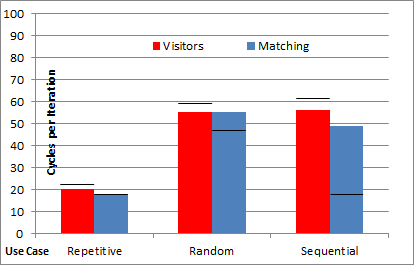
\includegraphics[width=0.47\textwidth]{VisitorsCompare.png}
  \caption{Sample timings for different benchmarks}
  \label{fig:VisitorsComparison}
\end{figure}

To give an idea about absolute timings of each of the benchmarks, 
Figure~\ref{fig:VisitorsComparison} presents a sample of performance numbers 
achieved by visitor design pattern and our open type switch when compiled with 
GCC 4.6.1 and ran in the diagnostic boot of OS on Windows Laptop. The actual 
bars show the timings without forwarding, while the black lines above and below 
each bar show where the corresponding bar would be in the presence of 
forwarding. It is easy to see that visitors generally become slower in the 
presence of forwarding due to extra call, while type switch becomes faster due 
to smaller jump table. As discussed, both timings are much smaller for 
repetitive benchmark due to hardware cache.

To give a broader view of how both techniques compare under different 
compiler/platform configurations, we also compare the performance of our 
solution relative to the performance of visitors in Figure~\ref{relperf}. The 
values are given as percentages of performance increase against the slower 
technique. Numbers in regular font represent cases where type switching was 
faster, while numbers in bold indicate cases where visitors were faster.

\begin{figure}[htbp]
\scriptsize
%\footnotesize
\begin{tabular}{@{}c@{ }@{}l@{ }||@{ }r@{ }|@{ }r@{ }|@{ }r@{ }|@{ }r@{ }|@{ }r@{ }|@{ }r@{ }||@{ }r@{ }|@{ }r@{ }|@{ }r@{ }|@{ }r@{ }|@{ }r@{ }|@{ }r@{ }}
\hline % ---------------------------------------------------------------
 &     & \multicolumn{6}{c||}{Open}     & \multicolumn{6}{c}{Closed}     \\
\hline % ---------------------------------------------------------------
 &     & \multicolumn{2}{@{}c@{}|}{G++} & \multicolumn{4}{@{}c@{}||}{MS Visual \Cpp{}} 
       & \multicolumn{2}{@{}c@{}|}{G++} & \multicolumn{4}{@{}c@{}}{MS Visual \Cpp{}} \\
\hline % ---------------------------------------------------------------
 &     & \multicolumn{1}{@{}c@{}|}{Lnx} & \multicolumn{1}{@{}c@{}|}{Win} 
       & \multicolumn{2}{@{}c@{}|}{PGO} & \multicolumn{2}{@{}c@{}||}{w/o PGO} 
       & \multicolumn{1}{@{}c@{}|}{Lnx} & \multicolumn{1}{@{}c@{}|}{Win} 
       & \multicolumn{2}{@{}c@{}|}{PGO} & \multicolumn{2}{@{}c@{}}{w/o PGO} \\
\hline % ---------------------------------------------------------------
 &     & \xV   & \xV   & \xV   & \xW   & \xV   & \xW   & \xV   & \xV   & \xV   & \xW   & \xV   &\xW     \\
\hline % ---------------------------------------------------------------
 & REP &\glNSPp&\gwNSPp&\VwNSPp&\VxNSPp&\vwNSPp&\vxNSPp&\glNSKp&\gwNSKp&\VwNSKp&\VxNSKp&\vwNSKp&\vxNSKp \\
 & SEQ &\glNSPq&\gwNSPq&\VwNSPq&\VxNSPq&\vwNSPq&\vxNSPq&\glNSKq&\gwNSKq&\VwNSKq&\VxNSKq&\vwNSKq&\vxNSKq \\
 & RND &\glNSPn&\gwNSPn&\VwNSPn&\VxNSPn&\vwNSPn&\vxNSPn&\glNSKn&\gwNSKn&\VwNSKn&\VxNSKn&\vwNSKn&\vxNSKn \\
\hline % ---------------------------------------------------------------
\multirow{3}{*}{\begin{sideways}{\tiny Forwarding}\end{sideways}}
 & REP &\glYSPp&\gwYSPp&\VwYSPp&\VxYSPp&\vwYSPp&\vxYSPp&\glYSKp&\gwYSKp&\VwYSKp&\VxYSKp&\vwYSKp&\vxYSKp \\
 & SEQ &\glYSPq&\gwYSPq&\VwYSPq&\VxYSPq&\vwYSPq&\vxYSPq&\glYSKq&\gwYSKq&\VwYSKq&\VxYSKq&\vwYSKq&\vxYSKq \\
 & RND &\glYSPn&\gwYSPn&\VwYSPn&\VxYSPn&\vwYSPn&\vxYSPn&\glYSKn&\gwYSKn&\VwYSKn&\VxYSKn&\vwYSKn&\vxYSKn \\
\hline % ---------------------------------------------------------------
\end{tabular}
\caption{Relative performance of type switching versus visitors. Numbers 
in regular font (e.g. \f{67}), indicate that our type switching is faster than 
visitors by corresponding percentage. Numbers in bold font (e.g. \s{18}), 
indicate that visitors are faster by corresponding percentage.}
\label{relperf}
\end{figure}

We can see that type switching wins by a good margin when implemented with tag switch as 
well as in the presence of at least one level of forwarding. Note that the 
numbers are relative, and thus the ratio depends on both the performance of 
virtual function calls and the performance of switch statements. Visual \Cpp{} was 
generating faster virtual function calls, while GCC was generating faster switch 
statements, which is why their relative performance seem to be much more 
favorable for us in the case of GCC.
Similarly, the code for x64 is only slower relatively: the actual time spent for 
both visitors and type switching was smaller than that for x86, but it was much 
smaller for visitors than type switching, which resulted in worse relative 
performance.

Lastly, the code on the critical path of our type switch implementation benefits 
significantly from branch hinting as some branches are much more likely than 
others. We use the branch hinting directives in GCC to guide the compiler, but, 
unfortunately, Visual \Cpp{} does not provide any similar facilities. Instead, 
Microsoft suggests using \emph{Profile-Guided Optimizations} (PGO) to achieve 
the same, which is why we list the results for Visual \Cpp{} both with and without 
profile-guided optimizations.
%The results without profile-guided optimizations can be 
%found in the accompanying technical report~\cite[\textsection 10]{TR}.
%The results of optimizing code created with Visual \Cpp{} by using profile 
%guided optimizations as currently Visual \Cpp{} does not have means for branch 
%hinting, which are supported by G++ and proven to be very effective in few 
%cruicial places. Profile guided optimization in Visual \Cpp{} lets compiler find 
%out experimentally what we would have otherwise hinted, even though this 
%includes other optimizations as well.

\subsection{Open vs. Closed Type Switch}
\label{sec:cmp}

With a few exceptions for x64, it can be seen from Figure~\ref{relperf} 
that the performance of the closed tag switch dominates the performance of the 
open type switch. We believe that the difference, often significant, is the 
price one pays for the true openness of the vtable pointer memoization solution. 

As we mentioned in \textsection\ref{sec:cotc}, the use of tags, even allocated 
by compiler, may require integration efforts to ensure that different DLLs have 
not reused the same tags. Randomization of tags, similar to a proposal of 
Garrigue~\cite{garrigue-98}, will not eliminate the problem and will surely 
replace jump tables in switches with decision trees. This will likely 
significantly degrade the numbers for the part of Figure~\ref{relperf} 
representing closed tag switch, since the tags in our experiments were all 
sequential. 

The reliance of a tag switch on static cast has severe limitations in the 
presence of multiple inheritance, and thus is not as versatile as open type 
switch. Overcoming this problem will either require the use of 
\code{dynamic_cast} or techniques similar to those used for vtable pointer 
memoization, which will likely degrade tag switch's performance numbers even 
further.

Note also that the approach used to implement open type switch can be used to 
implement both first-fit and best-fit semantics, while the tag switch is only suitable 
for best-fit semantics. Their complexity guarantees also differ: open type 
switch is constant on average, but slow on the first call with given subobject. 
Tag switch is logarithmic in the size of the class hierarchy 
(assuming a balanced hierarchy), including the first call. This last point can 
very well be seen in Figure~\ref{relperf}, where the performance of a closed solution
degrades significantly in the presence of forwarding, while the performance of an
open solution improves.

\subsection{Comparison with OCaml and Haskell}
\label{sec:ocaml}

We now compare our solution to the built-in pattern-matching facility of 
OCaml~\cite{OPM01} and Haskell~\cite{Haskell98Book}.  
In this test, we timed small OCaml and Haskell applications performing our sequential 
benchmark on an algebraic data type of 100 variants. Corresponding \Cpp{} 
applications were working with a flat class hierarchy of 100 derived classes. 
The difference between the \Cpp{} applications lies in the encoding used. Kind 
encoding is the same as Tag encoding, but it does not require substitutability, 
and thus can be implemented with a direct switch on tags. It is only supported 
through specialized syntax in our library as it differs from the Tag encoding 
only semantically.

%The optimized OCaml compiler \texttt{ocamlopt.opt} that we used to compile the code 
%can be based on different toolsets on some platforms, e.g. Visual \Cpp{} or GCC 
%on Windows. To make the comparison fair we had to make sure that the 
%same toolset was used to compile the \Cpp{} code. We ran the tests 
%on both of the machines described above using the following configurations: 

%\begin{itemize}
%\setlength{\itemsep}{0pt}
%\setlength{\parskip}{0pt}
%\item The tests on a Windows 7 laptop were all based on the \emph{Visual \Cpp{} toolset} 
%      and used \texttt{ocamlopt.opt} version 3.11.0.
%\item The tests on a Linux desktop were all based on the \emph{GCC toolset} and used 
%      \texttt{ocamlopt.opt} version 3.11.2
%\end{itemize}

%\noindent
We used optimizing OCaml compiler \texttt{ocamlopt.opt} version 3.11.0 working 
under the Visual \Cpp{} toolset as well as the Glasgow Haskell Compiler version 
7.0.3 (with -O switch) working under the MinGW toolset. All the tests were 
performed on the Windows 7 laptop.
The timing results presented in Figure~\ref{fig:OCamlComparison} are averaged 
over 101 measurements and show the number of seconds it took to perform a 
million decompositions within our sequential benchmark.

\begin{figure}[htbp]
  \centering
    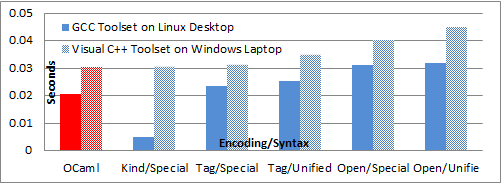
\includegraphics[width=0.47\textwidth]{OCamlComparison.png}
  \caption{Performance comparison of various encodings and syntax against OCaml code}
  \label{fig:OCamlComparison}
\end{figure}

%We can see that the use of specialized syntax on a closed/sealed hierarchy can 
%match the speed of, and even be four times faster than, the code generated by 
%the native OCaml compiler. Once we go for an open solution, we become about 
%30-50\% slower. 

\subsection{Dealing with real-world class hierarchies}
\label{sec:hierarchies}

We used a class hierarchy benchmark used previously in the literature to study efficiency of type 
inclusion testing and dispatching techniques~\cite{Vitek97,Krall97nearoptimal,PQEncoding,Ducournau08}. 
We use the names of the benchmarks from Vitek et al~\cite[Table 2]{Vitek97}, 
since the set of benchmarks we were working with was closest to that work.

While not all class hierarchies originated from \Cpp{}, for this experiment it 
was more important for us that the hierarchies were man-made. While converting 
the hierarchies into \Cpp{}, we had to prune inaccessible base classes (direct base  
class that is already an indirect base class) when used with repeated 
inheritance in order to satisfy semantic requirements of the \Cpp{}. We maintained 
the same number of virtual functions present in each class as well as the number 
of data members. The benchmarks, however, did not preserve the types of those.
The data in Figure~\ref{fig:benchmarks} shows various parameters of the class 
hierarchies in each benchmark, after their adoption to \Cpp{}. 

\begin{figure}[htbp]
\footnotesize
\begin{tabular}{@{ }l@{ }||@{ }l@{ }|@{ }r@{ }|@{ }r@{ }|@{ }r@{ }|@{ }r@{ }|@{ }r@{ }|@{ }r@{ }|@{ }l@{ }|@{ }r@{ }|@{ }r@{ }|@{ }r@{ }}
\hline % --------------------------------------------------------------------------------------------------
\multicolumn{1}{@{}c@{}||}{\multirow{2}{*}{\tiny{\textsc{Library}}}} & 
\multicolumn{1}{@{ }c@{ }|}{\multirow{2}{*}{\tiny{\textsc{Language}}}} & 
\multicolumn{1}{@{ }c@{ }|}{\multirow{2}{*}{\tiny{\textsc{Classes}}}} &
\multicolumn{1}{@{ }c@{ }|}{\multirow{2}{*}{\tiny{\textsc{Paths}}}} & 
\multicolumn{1}{@{ }c@{ }|}{\multirow{2}{*}{\tiny{\textsc{Height}}}} & 
\multicolumn{1}{@{ }c@{ }|}{\multirow{2}{*}{\tiny{\textsc{Roots}}}} & 
\multicolumn{1}{@{ }c@{ }|}{\multirow{2}{*}{\tiny{\textsc{Leafs}}}} & 
\multicolumn{1}{@{ }c@{ }|}{\multirow{2}{*}{\tiny{\textsc{Both}}}} & 
\multicolumn{2}{@{}c@{}|}{\tiny{\textsc{Parents}}} & 
\multicolumn{2}{@{}c@{}}{\tiny{\textsc{Children}}} \\ \cline{9-12}
     &                             &      &       &    &     &      &     & \multicolumn{1}{@{}c@{}|}{\tiny{\textsc{avg}}} & \multicolumn{1}{@{}c@{}|}{\tiny{\textsc{max}}} & \multicolumn{1}{@{}c@{}|}{\tiny{\textsc{avg}}} & \multicolumn{1}{@{}c@{}}{\tiny{\textsc{max}}} \\
\hline % --------------------------------------------------------------------------------------------------
 DG2 & \tiny{\textsc{Smalltalk}}   &  534 &   534 & 11 &   2 &  381 &   1 & 1    &  1 & 3.48 &  59 \\ % digitalk2         
 DG3 & \tiny{\textsc{Smalltalk}}   & 1356 &  1356 & 13 &   2 &  923 &   1 & 1    &  1 & 3.13 & 142 \\ % digitalk3         
 ET+ & \tiny{\textsc{\Cpp{}}}         &  370 &   370 &  8 &  87 &  289 &  79 & 1    &  1 & 3.49 &  51 \\ % et++              
 GEO & \tiny{\textsc{Eiffel}}      & 1318 & 13798 & 14 &   1 &  732 &   0 & 1.89 & 16 & 4.75 & 323 \\ % geode             
 JAV & \tiny{\textsc{Java}}        &  604 &   792 & 10 &   1 &  445 &   0 & 1.08 &  3 & 4.64 & 210 \\ % java              
 LOV & \tiny{\textsc{Eiffel}}      &  436 &  1846 & 10 &   1 &  218 &   0 & 1.72 & 10 & 3.55 &  78 \\ % lov-object-editor 
 NXT & \tiny{\textsc{Objective-C}} &  310 &   310 &  7 &   2 &  246 &   1 & 1    &  1 & 4.81 & 142 \\ % nextstep          
 SLF & \tiny{\textsc{Self}}        & 1801 & 36420 & 17 &  51 & 1134 &   0 & 1.05 &  9 & 2.76 & 232 \\ % self              
 UNI & \tiny{\textsc{\Cpp{}}}         &  613 &   633 &  9 & 147 &  481 & 117 & 1.02 &  2 & 3.61 &  39 \\ % unidraw           
%    &                             &   51 &    51 &  7 &   1 &   29 &   0 & 1.00 &  1 & 2.27 &   5 \\ % v1-collection     
%    &                             &   18 &    18 &  5 &   1 &   11 &   0 & 1.00 &  1 & 2.43 &   5 \\ % v1-magnitude      
%    &                             &  383 &   383 &  9 &   1 &  244 &   0 & 1.00 &  1 & 2.75 &  86 \\ % v1-object-nometa  
%    &                             &    9 &     9 &  5 &   1 &    4 &   0 & 1.00 &  1 & 1.60 &   2 \\ % v1-set            
%    &                             &   16 &    16 &  7 &   1 &    7 &   0 & 1.00 &  1 & 1.67 &   2 \\ % v1-stream         
%    &                             &   53 &    53 &  8 &   1 &   31 &   0 & 1.00 &  1 & 2.36 &   7 \\ % v1-visualcomponent
 VA2 & \tiny{\textsc{  }}          & 3241 &  3241 & 14 &   1 & 2582 &   0 & 1    &  1 & 4.92 & 249 \\ % visualage2.all    
 VA2 & \tiny{\textsc{  }}          & 2320 &  2320 & 13 &   1 & 1868 &   0 & 1    &  1 & 5.13 & 240 \\ % visualage2.kern   
 VW1 & \tiny{\textsc{Smalltalk}}   &  387 &   387 &  9 &   1 &  246 &   0 & 1    &  1 & 2.74 &  87 \\ % visualworks1      
 VW2 & \tiny{\textsc{Smalltalk}}   & 1956 &  1956 & 15 &   1 & 1332 &   0 & 1    &  1 & 3.13 & 181 \\ % visualworks2      
%    &                             &    6 &     9 &  4 &   2 &    1 &   0 & 1.50 &  2 & 1.20 &   2 \\ % vtbl              
\hline % --------------------------------------------------------------------------------------------------
\multicolumn{2}{r|}{\tiny{\textsc{Overalls}}} &15246 & 63963 & 17 & 298 &10877 & 199 & 1.11 & 16 & 3.89 & 323 \\ % Overalls
\hline % --------------------------------------------------------------------------------------------------
\end{tabular}
\caption{Benchmark Class Hierarchies}
\label{fig:benchmarks}
\end{figure}

The number of paths represents the number of distinct inheritance paths from the 
classes in the hierarchy to the roots of the hierarchy. This number reflects the number of possible subobjects in the 
hierarchy. The roots listed in the table are classes with no base classes. We 
will subsequently use the term \emph{non-leaf} to refer to the possible root of 
a subhierarchy. Leafs are classes with no children, while \emph{both} refers to 
utility classes that are both roots and leafs and thus neither have base nor 
derived classes. The average for the number of parents and the number of 
children were computed only among the classes having at least one parent or at 
least one child correspondingly.

With few useful exceptions, it generally makes sense to apply type switch only 
to non-leaf nodes of the class hierarchy. 71\% of the classes in the entire 
benchmarks suite were leaf classes. Out of the 4369 non-leaf classes 36\% were 
spawning a subhierarchy of only 2 classes (including the root), 15\% -- a 
subhierarchy of 3 classes, 10\% of 4, 7\% of 5 and so forth. 
Turning this into a cumulative distribution, $a\%$ of subhierarchies had more 
than $b$ classes in them, where:

%\noindent
\begin{tabular}
{l||@{ }c@{ }|@{ }c@{ }|@{ }c@{ }|@{ }c@{ }|@{ }c@{ }|@{ }c@{ }|@{ }c@{ }|@{ }c@{ }|@{ }c@{ }}
%{l||c|c|c|c|c|c|c|c|c}
$a$ & 1\% & 3\% & 5\% & 10\% & 20\% & 25\% & 50\% & 64\% & 100\% \\
\hline % --------------------------------------------------------------------------------------------------
$b$ & 700 & 110 & 50  & 20   & 10   & 7    & 3    & 2    & 1
\end{tabular}

%1\% of subhierarchies had more than 700 classes in them, 3\% of subhierarchies 
%had more than 110 classes, 5\% of subhierarchies had more than 50 classes, 10\% 
%of subhierarchies had more than 20 classes, 20\% of subhierarchies had more than 
%10 classes, 25\% of hierarchies had more than 7 classes, only 50\% of 
%hierarchies had more than 3 classes and 64\% -- more than 2.

\noindent
These numbers reflect the percentage of use cases one may expect in the real 
word that have a given number of case clauses in them.

For each non-leaf class $A$ we created a function performing a type switch on 
every possible derived class $D_i$ of it as well as itself. The function was 
then executed with every possible subobject $D_i\leftY\sigma_j\rightY A$ it can  
possibly be applied to, given the static type $A$ of the subject. It was 
executed multiple but the same number of times on each subobject to ensure 
uniformity on one side (since we do not have the data about the actual 
probabilities of each subobject in the benchmark hierarchies) as well as let the 
type switch infer the optimal parameters $k$ and $l$ of its cache indexing 
function $H_{kl}$. We then plotted a point in chart of Figure~\ref{fig:prob} 
relating 2 characteristics of each of the 4396 type switches tested: the optimal 
computed probability of conflict $p$ achieved by the type switch and the number 
of subobjects $n$ that came through that type switch. The actual frequencies of 
collisions were within one tenth of a percentage point of the computed 
probabilities, which is why we did not use them in the chart. To account for the 
fact that multiple experiments could have resulted in the same pair $(n,p)$, we 
use a shadow of each point to reflect somewhat the number of experiments 
yielding it.

\begin{figure}[htbp]
  \centering
    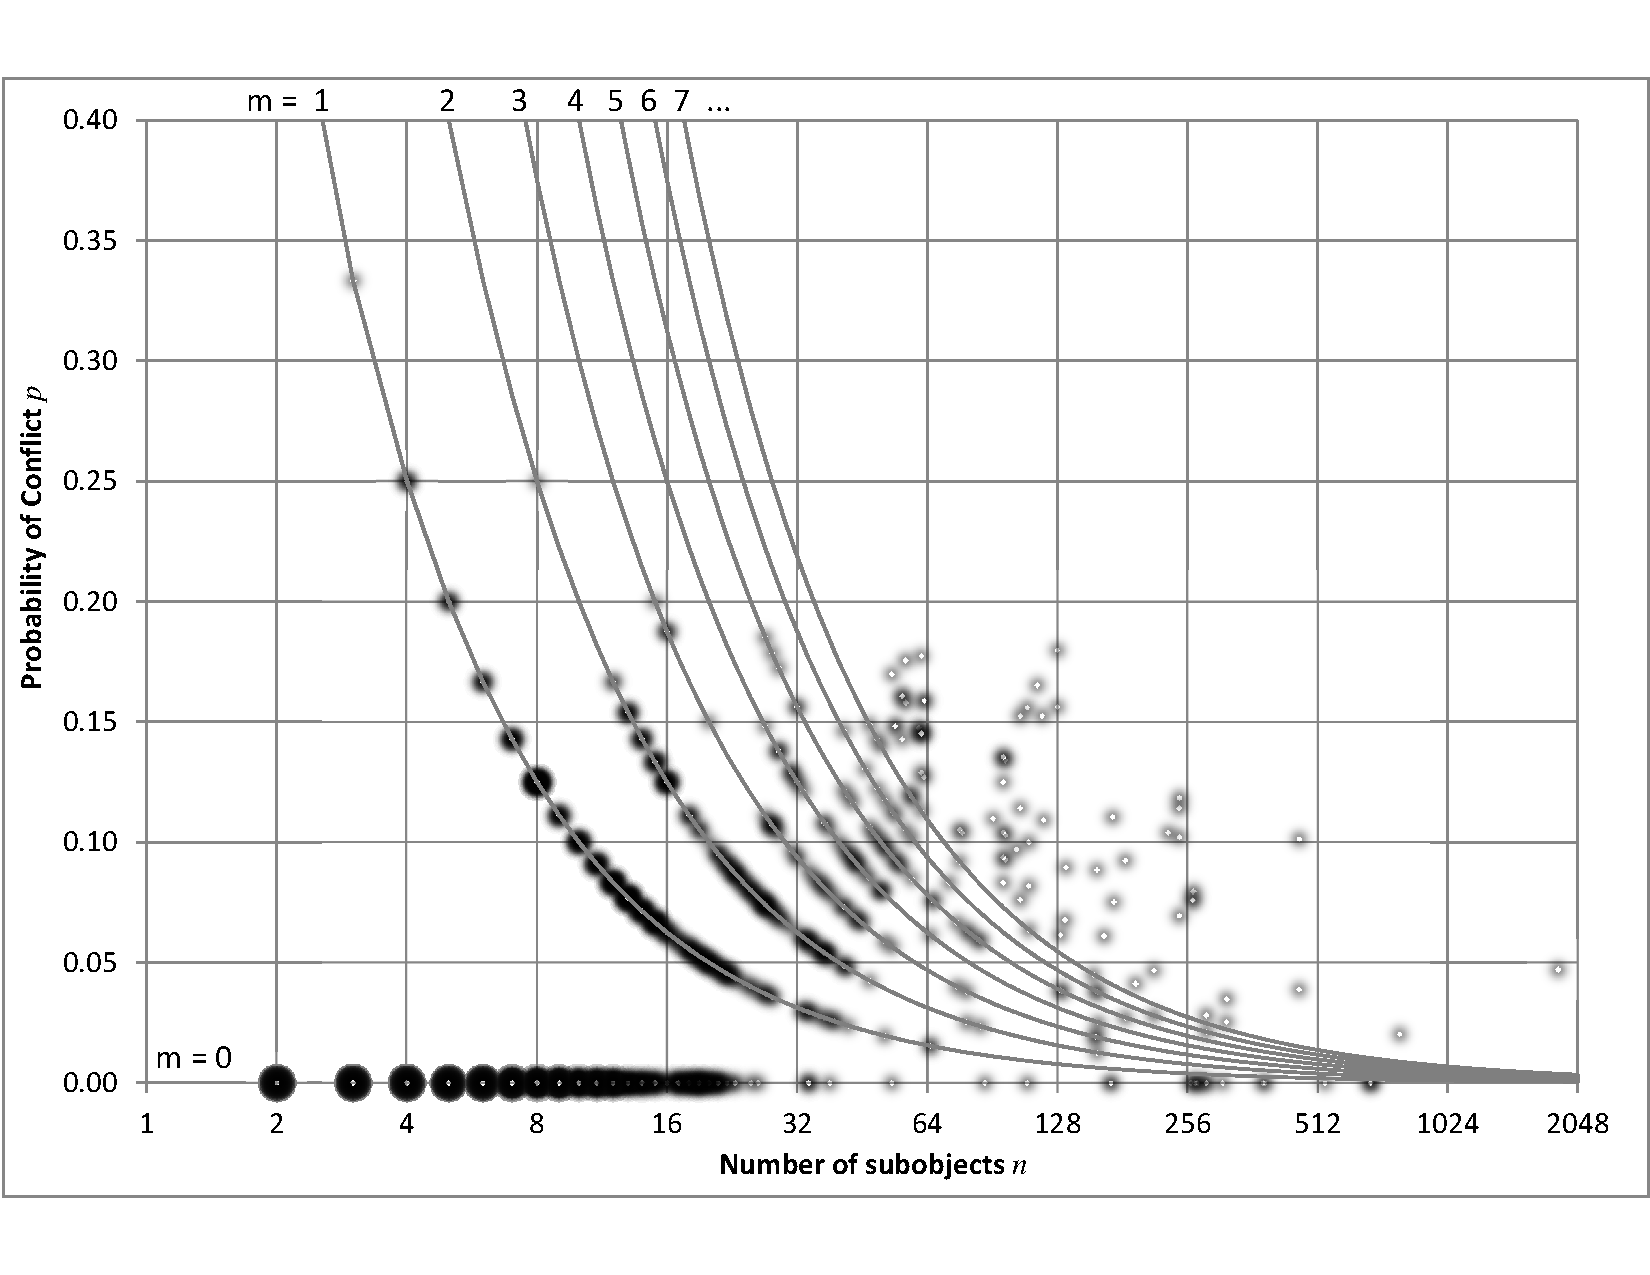
\includegraphics[width=0.49\textwidth]{ClassHierarchies.pdf}
  \caption{Probability of Conflict vs. Number of Subobjects in Hierarchy}
  \label{fig:prob}
\end{figure}

The curves on which the results of experiments line up correspond to the fact 
that under uniform distribution of $n$ subobjects, only a finite number of 
different values representing the probability of conflict $p$ is possible. In 
particular, all such values $p=\frac{m}{n}$, where $0 \le m < n$. The number $m$ 
reflects the number of subobjects an optimal cache indexing function $H_{kl}$ 
could not allocate their own entry for and we showed in \textsection\ref{sec:moc} 
that the probability of conflict under uniform distribution of $n$ subobjects 
depends only on $m$. The curves thus correspond to graphs of functions 
$y=\frac{m}{x}$ for different values of $m$. The points on the same curve (which 
becomes a line on a log-log plot) all share the same number $m$ of ``extra'' 
vtbl-pointers that optimal cache indexing function could not allocate individual 
entries for.

While it is hard to see from the chart, 87.5\% of all the points on the chart 
lay on the X-axis, which means that the optimal hash function for the 
corresponding type switches had no conflicts at all ($m=0$). In other words, only in 12.5\% 
of cases the optimal $H_{kl}^V$ for the set of vtbl-pointers $V$ coming through 
a given type switch had non-zero probability of conflict. Experiments laying on 
the first curve amount to 5.58\% of subhierarchies and represent the cases in 
which optimal $H_{kl}^V$ had only one ``extra'' vtbl-pointer ($m=1$). 2.63\% of 
experiments had $H_{kl}^V$ with 2 conflicts, 0.87\% with 3 and so forth as shown 
in Figure~\ref{fig:size}($K+1$).

\begin{figure}[htbp]
\small
\begin{tabular}
{@{}c@{}||@{}c@{}|@{}c@{}|@{}c@{}|@{}c@{}|@{}c@{}|@{}c@{}|@{}c@{}|@{}c@{}}
\hline % -------------------------------------------------------------------------
  $m$ &       0 &       1 &      2 &      3 &      4 &        5 &      6 & \textgreater 6 \\
\hline % -------------------------------------------------------------------------
  $K$ & 72.55\% & 12.27\% & 4.87\% & 2.61\% & 1.42\% & 0.94\% & 0.80\% & 4.55\% \\
\hline % -------------------------------------------------------------------------
$K+1$ & 87.50\% &  5.58\% & 2.63\% & 0.87\% & 0.69\% & 0.69\% & 0.30\% & 1.76\% 
\end{tabular}
\caption{Number of conflicts under different size constraints}
\label{fig:size}
\end{figure}

\noindent
In cases when the user is willing to trade performance for better space 
efficiency she may restrict $k$ to $[K,K]$ instead of $[K,K+1]$ as discussed in 
\textsection\ref{sec:moc}. We redid all the 4396 experiments under this 
restriction and obtained a similar histogram shown in Figure~\ref{fig:size}($K$).
The average probability of conflict over the entire set increased from 0.011 to 
0.049, while the maximum probability of conflict increased from 0.333 to 0.375. 
The average load factor of the cache increased from 75.45\% to 82.47\%. 

It is important to understand that the high ratio of cases in which the hash 
function could deliver perfect indexing does not indicate that the hash function 
we used is better than other hash functions. It does indicate instead that the 
values representing vtbl-pointers in a given application are not very random and 
are particularly suitable for such a hash function.

\subsection{Refactoring an existing visitors based application}
\label{sec:qualcmp}

For this experiment we have reimplemented a visitor based \Cpp{} pretty printer for 
Pivot\cite{Pivot09} using our pattern-matching library. Pivot's class hierarchy 
consists of 154 node kinds representing various entities in the \Cpp{} program. The 
original code had 8 visitor classes each handling 5, 7, 8, 10, 15, 17, 30 and 63 
cases, which we turned into 8 match statements with corresponding numbers of 
case clauses. Most of the rewrite was performed by sed-like replaces that 
converted visit methods into respective case-clauses. In several cases we had to 
manually reorder case-clauses to avoid redundancy as visit-methods for base classes 
were typically coming before the same for derived, while for type switching we 
needed them to come after. Redundancy checking support provided by our library 
was invaluable in finding out all such cases.

Both pretty printers were executed on a set of header files from the \Cpp{} 
standard library and the produced output of both program was byte-to-byte the same. 
We timed execution of the pretty printing phase (not including loading and termination 
of the application or parsing of the input file) and observed that on small 
files (e.g. those from C run-time library and few small \Cpp{} files) 
visitors-based implementation was faster because the total number of nodes in 
AST and thus calls did not justify our set-up calls. In particular, 
visitor-based implementation of pretty printer was faster on files of 44--588  
lines of code, with average 136 lines per those inputs, where visitors win. On 
these input files, it is faster by 1.17\%--21.42\% with an average speed-up of 
8.75\%. Open type switch based implementation of pretty printer was faster on 
files of 144--9851 lines of code, with average 3497 lines per those input files, 
where open type switch wins. On these inputs it is faster by 0.18\% -- 32.99\% 
with an average speed-up of 5.53\%.

Figure~\ref{fig:mem} shows memory usage as well as cache hits and misses for 
the run of our pretty printer on \code{<queue>} standard library 
header (it has the largest LOC after preprocessing in our test set).

\begin{figure}[htbp]
  \centering
    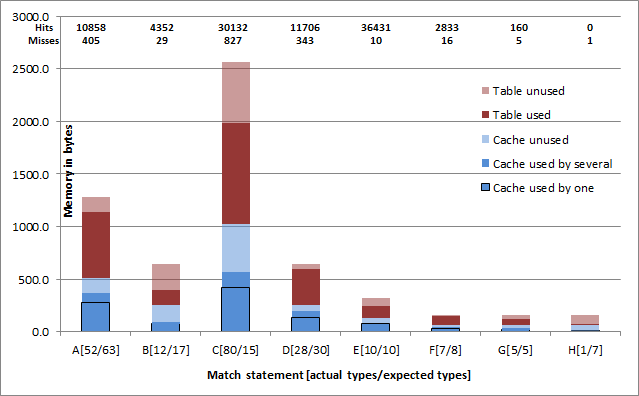
\includegraphics[width=0.49\textwidth]{Memory.png}
  \caption{Memory usage in real application}
  \label{fig:mem}
\end{figure}

The bars represent the total size of memory in bytes each of the 8 match 
statements (marked A-H) used. The info $[n/c]$ next to the letter indicates the 
actual number of different subobjects (i.e. vtbl-pointers) $n$ that came through 
that match statement, and the number of case clauses $c$ the match statement had 
(the library uses it as an estimate of $n$). $n$ is also the number of cases the 
corresponding match statement had to be executed sequentially (instead of a 
direct jump).

The blue part of each bar corresponds to the memory used by cache, while the 
maroon -- to the memory used by the hash table. The ratio of the non-opaque 
part of both colors to the entire part of that color indicates the load factors 
of cache and hash-table respectively. The black box additionally indicates the 
number of entries in the cache that are allocated for only one vtbl-pointer and 
thus never result in a cache miss. %The non-transparent part without black box 
%represents the percentage of vtbl-pointers that have to share their cache entry 
%with at least one other vtbl-pointer and thus may result in collisions during 
%access.

The actual number of hits and misses for each of the match statements is 
indicated on top of the corresponding column. The sum of them is the total 
number of calls made. %Hits indicate situation when we found entry in cache and 
%didn't have to make roundtrip to the hash-table to get it. Misses indicate the 
%number of cases during actual run we had to pick the entry from the hash table 
%and update the cache with it. 
The number of misses is always larger than or equal to $n$ since we need to 
execute the switch sequentially on each of them once in order to memoize the 
outcome.

The library always preallocates memory for at least 8 subobjects to avoid 
unnecessary recomputations of optimal parameters $k$ and $l$ -- this is the case 
with the last 3 match statements. In all other cases it allocates the 
memory proportional to $2^{K+1}$ where $2^{K-1} < \max(n,c) \le 2^{K}$. We make 
$c$ a parameter, because in a library setting $n$ is not known up front and 
estimating it with $c$ allows us to avoid unnecessary recomputations of $l$ and 
$k$ even further. 

The table does not have to be hash table and can be implemented with 
any other container i.e. sorted vector, map etc. that let us find quickly by a given 
vtbl-pointer the data associated with it. In fact we provide a slightly less 
efficient caching container that avoids the table altogether, thus significantly 
reducing the memory requirements instead.

%During this refactoring we have made several simplifications that became obvious 
%in pattern-matching code, but were not in visitors code because of control 
%inversion. Simplifications that were applicable to visitors code were eventually 
%integrated into visitors code as well to make sure we do not compare 
%algorithmically different code. In any case we were making sure that both 
%approaches regardless of simplifications were producing byte-to-byte the same 
%output as the original pretty printer we started from.

%The size of executable for pattern-matching approach was smaller than that for 
%visitors. So was also the source code. We extracted from both sources the 
%functionality that was common to them and placed it in a separate translation 
%unit to make sure it does not participate in the comparison. We kept all the 
%comments however that were eqaully applicable to code in either approach.
%
%Note that the visitors involved in the pretty printer above did not use 
%forwarding: since all the \Cpp{} constructs were handled by the printer, every 
%visit-method was overriden from those statically possible based on the static 
%type of the argument.

%Listing parameter for a case clause always causes access to member. Best hope is 
%that compiler will eliminate it if it is not needed. At the moment we do not 
%have means to detect empty macro arguments or \_.

%In general from our rewriting experience we will not recommend rewriting 
%existing visitor code with pattern matching for the simple reason that pattern 
%matching code will likely follow the structure already set by the visitors. 
%Pattern matching was most effective when writing new code, where we could design 
%the structure of the code having the pattern-matching facility in our toolbox.

\subsection{Limitations}
\label{sec:lim}

Currently the definition of each class used in a case clause must be visible to 
the compiler because \code{dynamic_cast} operator used in the type switch does 
not allow incomplete types as a target type. For particularly large type 
switches (e.g. \textgreater 1000 case clauses) this may easily reach some 
compiler limitations. Both GCC and Visual \Cpp{}, for example, could not generate 
object files for such translation units simply because the sheer size of v-tables 
and other compiler data in it were exceeding the limits. The problem is not 
specific to our technique though and allowing \code{dynamic_cast} on classes 
that were declared but not defined yet would solve the problem.

While it might be reasonable to expect from linkers to layout v-tables close 
to each other -- the property that makes our hashing function efficient -- they 
are not required to do so. We believe, nevertheless, that should our approach 
become popular through the library implementation, its compiler implementation 
will encourage compiler vendors to enforce the property in order to keep the 
type switching fast.


\section{Related Work} %%%%%%%%%%%%%%%%%%%%%%%%%%%%%%%%%%%%%%%%%%%%%%%%%%%%%%%%%
\label{sec:rw}

\emph{Extensible Visitors with Default Cases}~\cite[\textsection 
4.2]{Zenger:2001} attempt to solve the extensibility problem of visitors; 
however, the solution, after 
remapping it onto C++, has problems of its own. The visitation interface 
hierarchy can easily be grown linearly, but independent extensions by different  
authorities require developer's intervention. On top of the double dispatch the 
solution will incur two additional virtual calls and a dynamic cast for each 
level of visitor extension. The solution is simpler with virtual inheritance, 
which adds even more indirections.

L\"{o}h and Hinze proposed to extend Haskell's type system with open data types 
and open functions~\cite{LohHinze2006}. The solution allows top-level data types 
and functions to be marked as open with concrete variants and overloads defined 
anywhere in the program. The semantics of open extension is given by 
transformation into a single module, which assumes a whole-program view and thus 
is not an open solution unfortunately. Besides, open data types are extensible but not 
hierarchical, which avoids the problems discussed here.

Polymorphic variants in OCaml~\cite{garrigue-98} allow the addition of new 
variants as well as define subtyping on them. The subtyping, however, is not 
defined between the variants, but between combinations of them. 
This maintains disjointness between values from different variants and makes an 
important distinction between \emph{extensible sum types} like polymorphic 
variants and \emph{extensible hierarchical sum types} like classes. Our 
memoization device can be used to implement pattern matching on polymorphic 
variants.

\emph{Tom} is a pattern-matching compiler that can be used together with Java, C or 
Eiffel to bring a common pattern matching and term rewriting syntax into the 
languages~\cite{Moreau:2003}. In comparison to our approach, Tom has much bigger 
goals: the combination of pattern matching, term rewriting and strategies turns 
Tom into a fully fledged tree-transformation language. Its type patterns and \%match 
statement can be used as a type switch; however, Tom's handling of type 
switching is based on decision trees and an \code{instanceof}-like predicate, 
which are inefficient.

Pattern matching in Scala~\cite{Scala2nd} also support type switching through 
type patterns. The language supports extensible and hierarchical data types, but
their handling in a type switching constructs varies. Sealed classes are handled 
with an efficient switch over all tags, while extensible classes are similarly 
approached with a combination of an \code{InstanceOf} operator and a decision 
tree~\cite{EmirThesis}.

\section{Conclusions and Future Work} %%%%%%%%%%%%%%%%%%%%%%%%%%%%%%%%%%%%%%%%%%%%%%%%%%%%%%%%%%
\label{sec:cc}

Type switching is an open alternative to visitor design pattern that overcomes 
the restrictions, inconveniences, and difficulties in teaching and using, 
typically associated with it. Our implementation of it comes close or 
outperforms the visitor design pattern, which is true even in a library setting 
using a production-quality compiler, where the performance base-line is 
already very high.

%We describe three techniques that can be used to implement type switching, type 
%testing, pattern matching, predicate dispatching, and other facilities that 
%depend on the run-time type of an argument as well as demonstrate their efficiency.
%
%The \emph{Memoization Device} is an optimization technique that maps run-time values 
%to execution paths, allowing to take shortcuts on subsequent runs with the same 
%value. The technique does not require code duplication and in typical cases adds 
%only a single indirect assignment to each of the execution paths. It can be 
%combined with other compiler optimizations and is particularly suitable for use 
%in a library setting.
%
%The \emph{Vtable Pointer Memoization} is a technique based on memoization device that 
%employs uniqueness of virtual table pointers to not only speed up execution, but 
%also properly uncover the dynamic type of an object. This technique is a 
%backbone of our fast type switch as well as memoized dynamic cast optimization.
%
%The \emph{TPL Dispatcher} is yet another technique that can be used to 
%implement best-fit type switching on tagged classes. The technique has its pros 
%and cons in comparison to vtable pointer memoization, which we discuss in the paper.
%
%These techniques can be used in a compiler and library setting, and support well 
%separate compilation and dynamic linking. They are open to class extensions and 
%interact well with other C++ facilities such as multiple inheritance and 
%templates. The techniques are not specific to C++ and can be adopted in other 
%languages for similar purposes.
%
%Using these techniques, we implemented a library for efficient type switching 
%in C++. We used it to rewrite a code that relied heavily on 
%visitors, and discovered that the resulting code became much shorter, simpler, 
%and easier to maintain and comprehend.


\section{Future Work} %%%%%%%%%%%%%%%%%%%%%%%%%%%%%%%%%%%%%%%%%%%%%%%%%%%%%%%%%%
\label{sec:fw}

The current implementation of our library relies on static variables and global 
state, which will have problems in a multi-threaded environment. Efficient 
multi-threaded implementation is the first task on our list. 

We would also like to experiment with other kinds of cache indexing functions in 
order to decrease the frequency of conflicts, especially those coming from the use 
of dynamically-linked libraries.

The match statement that we presented here deals with only one scrutiny at the 
moment, but we believe that our memoization device, along with the v-table pointer memoization 
technique we presented, can cope reasonably efficiently with multiple scrutinies. 
Their support will make our library more general by addressing asymmetric 
multiple dispatch.


\acks

We would like to thank Xavier Leroy and Luc Maranget for valuable feedback and 
suggestions for improvements on the initial idea, Gregory Berkolaiko for ideas 
related to minimization of conflicts, Jaakko Jarvi for assistance in comparison 
to other languages, Andrew Sutton, Peter Pirkelbauer and Abe Skolnik for helpful 
discussions and comments to numerous rewrites of this paper. 
We also benefitted greatly from insightful comments by anonymous reviewers on 
earlier revisions of this work. We would also like to thank Karel Driesen for 
letting us use his class hierarchies benchmark for this work.

\bibliographystyle{abbrvnat}
\bibliography{mlpatmat}
\end{document}
